%%!TEX encoding = UTF-8 Unicode

% Several lines in file have comments suggesting common packages for the
% typical thesis in informatics or electronics developed at UA
% uncomment/comment the lines as required for your work
% Before each optional line you will have a small comment

% According to UA rules, font size should range from 10 to 12pt.
\documentclass[11pt,a4paper,oneside,onecolumn]{memoir}

\listfiles
\fixpdflayout

\usepackage[utf8]{inputenc}

% Select Computer Modern Typewritter (For bold ttfamily in listings)
\usepackage{lmodern}
% OR... Bera Mono
%\usepackage[scaled]{beramono} % TTT Font
%\usepackage{anyfontsize} % As the name says...

\usepackage[T1]{fontenc}

\usepackage{tabularx}

% Enable for for Overleaf support
\usepackage{ifthen}
\def\useoverleaf{1}  % change to non-zero (for instance, 1) to enable it

\makeatletter
\newcommand{\makecoverfile}[0]{%
  \immediate\write18{latexmk -pdf cover.tex}%
}
\makeatother

% For PDF merging
\usepackage{pdfpages}

% Set DPI to 300
\pdfpxdimen=\dimexpr 1in/300\relax

% Allow the use of a larger number of packages
\usepackage{morewrites} 

% For English and Portuguese languages
% Portuguese will be the default.
% Uncomment \setlanguage below to change it
\usepackage[english,portuguese]{babel}

% Uncomment to use a custom date format
%\usepackage{datetime}
%\newdateformat{thesisdate}{\monthname[\THEMONTH] \THEYEAR} % Month Year

% Make pdf look better
\usepackage{microtype} 

% Uncomment to enable floats on facing pages
%\usepackage{dpfloat}

% Side by side figures
% Eg. Fig 1a, Fig 1b
\usepackage[hang,small,bf]{caption}
%\let\tion\undefined
%\let\subfloat\undefined
\usepackage{subcaption}

%\RequirePackage{textcase}

% Dropped Caps
%\usepackage{lettrine}

% Configure Hyperlink color
% As a matter or style, you may use this to enable/disable color boxes on links
%\usepackage[breaklinks=true,colorlinks=false,linkcolor=blue]{hyperref}
% Or use the default values provided by the hyperref package
\usepackage{hyperref}

% Redefine section names according to your preference
%\def\sectionautorefname{Section}
%\def\chapterautorefname{Chapter}
%\def\figureautorefname{Figure}
%\def\listingautorefname{Listing}
%\def\tableautorefname{Table}

% Redefine code boxes
\ifthenelse{\equal{\useoverleaf}{0}}
{\usepackage[outputdir=build]{minted}}
{\usepackage{minted}}%

\addto\captionsportuguese{%
  \renewcommand\listingscaption{Código}
}
\fvset{fontsize=\footnotesize} % Make Code blocks smaller than text
\usepackage{csquotes}

% Add support for PDF Comments
\usepackage{comment}
\ifthenelse{\equal{\useoverleaf}{0}}
{\usepackage{pdfcomment}}{}
\usepackage{bookmark} % New Bookmarks

% For Multiple columns in Glossary
\usepackage{multicol}

% Add support for Math symbols
\usepackage{amsmath}
\usepackage{amssymb}

% Add support for graphics
\usepackage{graphicx}

% Add support for Colors
\usepackage{xcolor}

% Add support for the Euro symbol
\usepackage{eurosym}

% Add support for missingfigure and todo
\usepackage{todonotes}

% Setup bibliography with Biber using IEEE style for proper UTF-8 support
\usepackage[backend=biber, style=ieee, sorting=none, natbib=true, mincitenames=1, maxcitenames=2]{biblatex}
\bibliography{bib/references.bib}

% Use acronyms
\usepackage[printonlyused]{acronym} % For acronyms

% Indenting the first paragraph after section start
\usepackage{indentfirst}

% For fixing listoflistings with memoir
\usepackage{xparse}

% Uncomment the next lines to enable chart support through pgf and tikz
% This may require you to install further packages in your Tex system
%\usepackage[version=0.96]{pgf}
%\usepackage{tikz}

% UML support
%\usepackage{pgf-umlsd}

% Trees, Arrows, Mindmaps and other popular objects
%\usetikzlibrary{arrows,shadows,trees,shapes,decorations,automata,backgrounds,petri,mindmap} % for pgf-umlsd

% Package to master SI units
\usepackage[detect-weight=true, binary-units=true]{siunitx}
% For Electric Circuits
%\sisetup{load-configurations = binary}

% Set Voltage direction accordingly
% Option : oldvoltagedirection,nooldvoltagedirection,RPvoltages,EFvoltages
% More information at: https://mirrors.ibiblio.org/CTAN/graphics/pgf/contrib/circuitikz/doc/circuitikzmanual.pdf
% By default this template is using the Old Voltage Direction
%\usepackage[oldvoltagedirection,american,cuteinductors,smartlabels]{circuitikz}
%\usetikzlibrary{calc}
%\ctikzset{bipoles/thickness=1}
%\ctikzset{bipoles/length=0.8cm}
%\ctikzset{bipoles/diode/height=.375}
%\ctikzset{bipoles/diode/width=.3}
%\ctikzset{tripoles/thyristor/height=.8}
%\ctikzset{tripoles/thyristor/width=1}
%\ctikzset{bipoles/vsourceam/height/.initial=.7}
%\ctikzset{bipoles/vsourceam/width/.initial=.7}
%\tikzstyle{every node}=[font=\small]
%\tikzstyle{every path}=[line width=0.8pt,line cap=round,line join=round]

% For inline TT text (e.g. code snippets)
\usepackage{verbatim}

% Frames around figures and allow force placement
\usepackage{float}

% Configure Float style
%\floatstyle{boxed}
%\restylefloat{table}
%\restylefloat{figure}
%\restylefloat{lstlisting}

% For test purposes you may use the lipsum package to create dummy text
\usepackage{lipsum} % REMOVE

%Keep floats inside section!
\usepackage[section]{placeins}
\let \oldsubsubsection \subsubsection
\renewcommand{\subsubsection}[2][]{
  \FloatBarrier
  \oldsubsubsection#1{#2}
}
\let \oldsubsection \subsection
\renewcommand{\subsection}[2][]{
  \FloatBarrier
  \oldsubsection#1{#2}
}
\let \oldsection \section
\renewcommand{\section}[2][]{
  \FloatBarrier
  \oldsection#1{#2}
}
\let \oldchapter \chapter
\renewcommand{\chapter}[2][]{
  \FloatBarrier
  \oldchapter#1{#2}
}



% Use the built-in division styling
\headstyles{memman}

% Include subsections in the TOC
\settocdepth{subsection}

% Numbering down to subsections as well
\setsecnumdepth{subsection}

% extra index for first lines
\makeindex[lines]

% Margins for University of Aveiro Thesis
\setlrmarginsandblock{3cm}{2.5cm}{*}
\setulmarginsandblock{3cm}{3cm}{*}
\checkandfixthelayout

% Or select your custom spacing to make any ajustment
%\addtolength{\parskip}{0.5\baselineskip}
\linespread{1.5}

\newcommand\mainmatterWithoutReset
{\edef\temppagenumber{\arabic{page}}%
  \mainmatter
  \setcounter{page}{\temppagenumber}%
}

\usepackage{listings}

\definecolor{codegreen}{rgb}{0,0.6,0}
\definecolor{codegray}{rgb}{0.5,0.5,0.5}
\definecolor{codepurple}{rgb}{0.58,0,0.82}
\definecolor{backcolour}{rgb}{0.95,0.95,0.92}

\lstdefinestyle{code}{
    backgroundcolor=\color{backcolour},   
    commentstyle=\color{codegreen},
    keywordstyle=\color{magenta},
    numberstyle=\tiny\color{codegray},
    stringstyle=\color{codepurple},
    basicstyle=\ttfamily\footnotesize,
    breakatwhitespace=false,         
    breaklines=true,                 
    captionpos=b,                    
    keepspaces=true,                   
    numbersep=5pt,                  
    showspaces=false,                
    showstringspaces=false,
    showtabs=false,                  
    tabsize=2
}

\lstset{style=code}


%%%%%%%%%%%%%%%%%%%%%%%%%%%%%%%%%%%%%%%%%%%%%%%%%%
% Document begins here
%%%%%%%%%%%%%%%%%%%%%%%%%%%%%%%%%%%%%%%%%%%%%%%%%%

\begin{document}

% Fix the numbering scheme by having a ghost style for page numbering
\pagenumbering{Alph}

\ifthenelse{\equal{\useoverleaf}{0}}{}{\makecoverfile{}}%
\setcounter{page}{0}
\includepdf[pages=-]{cover.pdf}

% Uncomment to enable English
\selectlanguage{english}

% Front matter

%Custom Chapter style named `thesis`
\makechapterstyle{thesis}{% Based on ell
  \chapterstyle{default}
  \renewcommand*{\chapnumfont}{\normalfont\sffamily}
  \renewcommand*{\chaptitlefont}{\normalfont\Huge\sffamily}
  \settowidth{\chapindent}{\chapnumfont 111}
  \renewcommand*{\chapterheadstart}{\begingroup
    \vspace*{\beforechapskip}%
    \begin{adjustwidth}{}{-\chapindent}%
    \hrulefill
    \smash{\rule{0.4pt}{15mm}}
    \end{adjustwidth}\endgroup}
  \renewcommand*{\printchaptername}{}
  \renewcommand*{\chapternamenum}{}
  \renewcommand*{\printchapternum}{%
    \begin{adjustwidth}{}{-\chapindent}
    \hfill
    \raisebox{10mm}[0pt][0pt]{\fontsize{30}{25}\selectfont\chapnumfont \thechapter}%
                              \hspace*{1em}
    \end{adjustwidth}\vspace*{-3.0\onelineskip}}
  \renewcommand*{\printchaptertitle}[1]{%
    \vskip\onelineskip
    \raggedleft {\chaptitlefont ##1}\par\nobreak\vskip 4\onelineskip}}


% Select chapter style from existing or select custom
%\chapterstyle{thesis} % Others: dowding, demo2, dash, chappell, brotherton, bianchi, ger, madsen, tatcher, veelo,indexes)
% thesis can also be used as defined previously
% Check the memoir documentation for the available themes
% Default is veelo
\chapterstyle{veelo}
\makeoddfoot{plain}{}{\thepage}{} % Added by André Zúquete to fix a page numbering issue on the veelo chapter style

% Select Page style
\pagestyle{plain}

% If you feel adventurous you can also define all aspects of your theme
% Use either this input or the chapterstyle before
% % Rules
\newcommand{\thinRule}{\rule{\textwidth}{0.25pt}}

% Customize heading appearances
% Define styles
\newcommand{\partSize}{\Huge}
\newcommand{\partStyle}{\lsstyle\scshape}
\newcommand{\chapterSize}{\Huge}
\newcommand{\chapterStyle}{\lsstyle\scshape}
\newcommand{\chapterAfter}{}
\newcommand{\sectionSize}{\Large}
\newcommand{\sectionStyle}{\scshape\MakeTextLowercase}
\newcommand{\subsectionSize}{\large}
\newcommand{\subsectionStyle}{\scshape\MakeTextLowercase}
\newcommand{\subsubsectionSize}{\large}
\newcommand{\subsubsectionStyle}{\scshape\MakeTextLowercase}
\newlength{\partNumSizePt}
\setlength{\partNumSizePt}{60pt}
\newlength{\chapterNumSizePt}
\setlength{\chapterNumSizePt}{60pt}
\newcommand{\partNumSize}{%
  \fontsize{\partNumSizePt}{1.2\partNumSizePt}\selectfont%
}
\newcommand{\partNumStyle}{\partChapterNumColor}
\newcommand{\chapterNumSize}{%
  \fontsize{\chapterNumSizePt}{1.2\chapterNumSizePt}\selectfont%
}
\newcommand{\chapterNumStyle}{\partChapterNumColor}

% Customize parts
\renewcommand{\partnamefont}{\partSize\partStyle}
\renewcommand{\partnumfont}{\partNumSize\partNumStyle}
\renewcommand{\printpartname}{}
\renewcommand{\printparttitle}[1]{%
  \normalfont\normalcolor\partnamefont #1
}

% Customize chapters
\makeatletter
\setlength{\beforechapskip}{30pt}
\renewcommand*{\chapterheadstart}{\vspace*{\beforechapskip}}
\setlength{\afterchapskip}{3ex}
\setlength{\midchapskip}{3ex}
\renewcommand*{\chapnamefont}{%
  \Large\flushright\chapterStyle\partChapterNumColor%
}
\renewcommand*{\chapnumfont}{\chapterNumSize\chapterNumStyle}
\renewcommand*{\chaptitlefont}{%
  \normalfont\flushleft\normalcolor\chapterSize\chapterStyle%
}
\renewcommand*{\printchaptername}{%
  \chapnamefont\MakeTextLowercase{\@chapapp}%
}
\renewcommand*{\chapternamenum}{\quad}
\renewcommand*{\printchapternum}{%
%  \chapnumfont\textls[-75]{\classicstylenums{\thechapter}}%
 \chapnumfont\textls[-75]{\thechapter}%

}
\renewcommand*{\printchaptertitle}[1]{%
  \chaptitlefont #1
  \chapterAfter
}
\makeatother
% Customize sections and subsections
\setsecnumformat{\csname my#1\endcsname\quad}
\setsecheadstyle{\sectionSize\sectionStyle}
\newcommand{\mysection}{{\thesection}}
\setlength{\beforesecskip}{3em}


\setsubsecheadstyle{\subsectionSize\subsectionStyle}
\newcommand{\mysubsection}{{\normalfont\subsectionSize\thesubsection}}
\setlength{\beforesubsecskip}{3em}

\setsubsubsecheadstyle{\subsubsectionSize\subsubsectionStyle}
\newcommand{\mysubsubsection}{{\normalfont\subsubsectionSize\thesubsubsection}}
\setlength{\beforesubsubsecskip}{2em}

% Customize "Table of ..." appearance
% Customize headings
\newcommand{\renewPrintXTitle}[1]{%
  \renewcommand{#1}[1]{%
    \printchaptertitle{##1}%
  }%
}
\renewPrintXTitle{\printtoctitle}
\renewPrintXTitle{\printlottitle}
\renewPrintXTitle{\printloftitle}

% Customize ToC headings
\renewcommand{\cftpartfont}{\partChapterNumColor\partStyle}
\renewcommand{\cftchapterfont}{\chapterStyle}
\renewcommand{\cftsectionfont}{}
\renewcommand{\cftsubsectionfont}{}
\renewcommand{\cftfigurefont}{}
\renewcommand{\cfttablefont}{}
\newcommand{\cftlstlistingfont}{}

% Increase number width
\newlength{\cftNumWidthIncrease}
\setlength{\cftNumWidthIncrease}{0.25em}
\addtolength{\cftpartnumwidth}{\cftNumWidthIncrease}
\addtolength{\cftchapternumwidth}{\cftNumWidthIncrease}
\addtolength{\cftsectionindent}{\cftNumWidthIncrease}
\addtolength{\cftsubsectionindent}{\cftNumWidthIncrease}
% No leader dots
%\renewcommand*{\cftpartdotsep}{\cftnodots}
%\renewcommand*{\cftchapterdotsep}{\cftnodots}
%\renewcommand*{\cftsectiondotsep}{\cftnodots}
%\renewcommand*{\cftsubsectiondotsep}{\cftnodots}
%\renewcommand*{\cftfiguredotsep}{\cftnodots}
%\renewcommand*{\cfttabledotsep}{\cftnodots}
%\newcommand*{\cftlstlistingdotsep}{\cftnodots}
% Set page numbers immediately after entry text
\newcommand{\tocEntryPageSep}{\hspace{1em}}
\renewcommand{\cftpartleader}{\cftdotfill{\cftdotsep}}
%\renewcommand{\cftpartafterpnum}{\cftparfillskip}
%\renewcommand{\cftchapterleader}{\tocEntryPageSep}
\renewcommand{\cftchapterleader}{\cftdotfill{\cftdotsep}}
%\renewcommand{\cftchapterafterpnum}{\cftparfillskip}
\renewcommand{\cftsectionleader}{\cftdotfill{\cftdotsep}}
%\renewcommand{\cftsectionafterpnum}{\cftparfillskip}
\renewcommand{\cftsubsectionleader}{\cftdotfill{\cftdotsep}}
%\renewcommand{\cftsubsectionafterpnum}{\cftparfillskip}
\renewcommand{\cftfigureleader}{\cftdotfill{\cftdotsep}}
%\renewcommand{\cftfigureafterpnum}{\cftparfillskip}
\renewcommand{\cfttableleader}{\cftdotfill{\cftdotsep}}
%\renewcommand{\cfttableafterpnum}{\cftparfillskip}
\newcommand{\cftlstlistingleader}{\cftdotfill{\cftdotsep}}
%\newcommand{\cftlstlistingafterpnum}{\cftparfillskip}
% Customize page numbers
\newcommand{\tocPageStyle}{\tocPageColor}
\renewcommand{\cftpartpagefont}{\tocPageStyle}
\renewcommand{\cftchapterpagefont}{\tocPageStyle}
\renewcommand{\cftsectionpagefont}{\tocPageStyle}
\renewcommand{\cftsubsectionpagefont}{\tocPageStyle}
\renewcommand{\cftfigurepagefont}{\tocPageStyle}
\renewcommand{\cfttablepagefont}{\tocPageStyle}
\newcommand{\cftlstlistingpagefont}{\tocPageStyle}

% Abstract
% Remove indents around abstract text
\setlength{\absleftindent}{0pt}
\setlength{\absrightindent}{0pt}
% Change font size to conform with the rest of the document text
\renewcommand{\abstracttextfont}{\normalsize}

% Customize headers and footers including page numbers
\newcommand{\hfTextSize}{\footnotesize}
\newcommand{\headTextStyle}{\lsstyle\scshape\MakeTextLowercase}
\nouppercaseheads
\makeevenhead{headings}%
             {\hfTextSize\thepage}%
             {}%
             {\hfTextSize\headTextStyle\leftmark}
\makeevenhead{plain}%
             {\hfTextSize\thepage}%
             {}%
             {\hfTextSize\headTextStyle\leftmark}
\makeoddhead{headings}%
            {\hfTextSize\headTextStyle\rightmark}%
            {}%
            {\hfTextSize\thepage}
\makeoddhead{plain}%
            {\hfTextSize\headTextStyle\rightmark}%
            {}%
            {\hfTextSize\thepage}


% Customize captions
\newcommand{\captionSize}{\small}
\newcommand{\captionStyle}{\scshape}
\newcommand{\captionWidthRatio}{0.9}

\captionnamefont{\captionSize\captionStyle}
\captiontitlefont{\captionSize}
\captiondelim{ -- }
\captiontitlefinal{}
\changecaptionwidth
%\captionwidth{\captionWidthRatio\textwidth}

% Define colors
%\newcommand{\titleColor}{\color[rgb]{0.616, 0.0627, 0.176}}
\newcommand{\titleColor}{\color[rgb]{0,0,0}}

\newcommand{\partChapterNumColor}{\titleColor}
\newcommand{\dropCapColor}{\titleColor}
%\newcommand{\tocPageColor}{\color[rgb]{0.0980, 0.329, 0.651}}

\newcommand{\tocPageColor}{\color[rgb]{0, 0,0}}
\definecolor{shade0}{rgb}{1.0 , 1.0 , 1.0 }
\definecolor{shade1}{rgb}{0.9 , 0.9 , 0.9 }
\definecolor{shade2}{rgb}{0.8 , 0.8 , 0.8 }
\definecolor{shade3}{rgb}{0.65, 0.65, 0.65}
\definecolor{shade4}{rgb}{0.45, 0.45, 0.45}
\definecolor{shade5}{rgb}{0.0 , 0.0 , 0.0 }



%Exclude sub figures from List of Figures
%\captionsetup[subfloat]{list=no}

% Texts
\newenvironment{introduction}
{%
  \begin{minipage}{\textwidth}%
   \itshape%
}
{%
  \end{minipage}%
  \par\addvspace{2\baselineskip plus 0.2\baselineskip minus 0.2\baselineskip}%
}

\frontmatter

\tightlists
\midsloppy
\raggedbottom

\setcounter{tocdepth}{4} %subsections are added to the TOC
\setcounter{secnumdepth}{4} %subsubsections are numbered

% Initial document tables start here: TOC, LOF, LOT, Glossary
% Table of contents with slightly smaller font
{\small\tableofcontents}

% List of figures with slightly smaller font
\clearpage
{\small\listoffigures}

% List of tables with slightly smaller font
\clearpage
{\small\listoftables}

% Fix for Listings with memoir

\RenewDocumentCommand \chapter { s O{#3} m }{%
  \FloatBarrier
  \IfValueTF{#1}  % if optional star is seen
    {\oldchapter*{#2}}
    {\oldchapter#1{#2}}
}

\renewcommand{\listingscaption}{Code}
\renewcommand{\listoflistingscaption}{List of Code Snippets}
\clearpage
{\small\listoflistings}
\addcontentsline{toc}{chapter}{\listoflistingscaption}

% Reset Chapters
\renewcommand{\chapter}[2][]{
  \FloatBarrier
  \oldchapter#1{#2}
}

% Print Glossary
\clearpage
{\small\chapter{Glossary}

\footnotesize
\SingleSpacing

\begin{multicols}{2}
\begin{acronym}[AAAAAA]
\acro{3G}[3G]{third-generation}
\acro{3GPP}[3GPP]{3rd Generation Partnership Project}
\acro{4G}[4G]{fourth-generation}
\acro{5G}[5G]{fifth-generation}
\acro{5G-AKA}[5G-AKA]{5G - Authentication and Key Management}
\acro{5GC}[5GC]{5G Core}
\acro{AV}[AV]{Authentication Vector}
\acro{CP}[CP]{Control Plane}
\acro{EAP}[EAP]{Extensible Authentication Protocol}
\acro{EAP-AKA'}[EAP-AKA']{EAP - Authentication and Key Management}
\acro{EAP-TLS}[EAP-TLS]{EAP - Transport Layer Security}
\acro{eMBB}[eMBB]{enhanced mobile broadband}
\acro{eNodeB}[eNodeB]{evolved Node B}
\acro{EPS}[EPS]{Evolved Packet System}
\acro{EPS-AKA}[EPS-AKA]{Evolved Packet System - Authentication and Key Management}
\acro{GUTI}[GUTI]{Globally Unique Temporary Identity}
\acro{HSS}[HSS]{Home Subscriber Server}
\acro{HN}[HN]{Home Network}
\acro{IMSI}[IMSI]{International Mobile Subscriber Identity}
\acro{IP}[IP]{Internet Protocol}
\acro{MAC}[MAC]{medium access control}
\acro{MMe}[MMe]{Mobility Management Entity}
\acro{mMTC}[mMTC]{massive machine-type communications}
\acro{NAI}[NAI]{Network Access Identifier}
\acro{N5GC}[N5GC]{Non-5G-Capable}
\acro{NFV}[NFV]{Network Functions Virtualization}
\acro{NR}[NR]{5G New Radio}
\acro{SBA}[SBA]{Service Based Architecture}
\acro{SDN}[SDN]{Software Defined Network}
\acro{SEAF}[SEAF]{Security Anchor Function}
\acro{SN}[SN]{Serving Network}
\acro{SUCI}[SUCI]{Subscriber Concealed Identifier}
\acro{SUPI}[SUPI]{Subscription Permanent Identifier}
\acro{TSN}[TSN]{time-sensitive networks}
\acro{UE}[UE]{User Equipment}
\acro{UP}[UP]{User Plane}
\acro{uRLLC}[uRLLC]{ultra-reliable low-latency communications}
\acro{USIM}[USIM]{Universal Subscriber Identity Module}
\acro{WBA}[WBA]{Wireless Broadband Alliance}
\end{acronym}
\end{multicols}

}

%%%%%%%%%%%%%%%%%%%%%%%%%%%%%%%%%%%%%%%%%%%%%%%%%%%%%%%
% Main document starts here
%%%%%%%%%%%%%%%%%%%%%%%%%%%%%%%%%%%%%%%%%%%%%%%%%%%%%%%

\mainmatter

% Line spacing: 1.5 pt 
\OnehalfSpacing

%%%%%%%%%%%%%%%%%%%%%%%%%%%%%%%%%%%%%%%%%%%%%%%%%%%%%%%
% Start of Thesis text 
%%%%%%%%%%%%%%%%%%%%%%%%%%%%%%%%%%%%%%%%%%%%%%%%%%%%%%%

% Uncomment to add further chapters
\chapter{Introduction}%
\label{chapter:introduction}

\begin{introduction}
This chapter summarizes the challenges and significance of integrating Wi-Fi-only devices into the 5G core network, highlighting the limitations of current standards and the need for innovative solutions to enable seamless connectivity and authentication.
\end{introduction}

\section{Background and Context}

% Introduce 5G as a significant advancement in wireless technology, highlighting its core features such as higher speeds, lower latency, and support for diverse use cases (e.g., enhanced mobile broadband, massive machine-type communications, ultra-reliable low-latency communications).

In recent years, \ac{5G} wireless technology has revolutionized telecommunications. It offers higher bandwidth, faster speeds, and lower delays, supporting use cases like \ac{eMBB}, \ac{mMTC}, and \ac{uRLLC}.

Additionally, it is transforming private networks, which have traditionally relied on legacy wired or wireless (WLAN) Ethernet. Features like tighter security, higher reliability, and \ac{TSN} are crucial to meeting Industry 4.0 requirements for wireless connectivity. However, how can the industry bridge the gap between existing \ac{N5GC} devices, which current networks rely on, and new \acp{5GC}?

% Briefly describe the Service Based Architecture of 5G, emphasizing the incorporation of Network Functions Virtualization (NFV) and Software Defined Networking (SDN).
% Mention the various access nodes supported by the 5G system, including native 5G-NR and LTE accesses, and non-3GPP interworking functions.

\ac{5G} is not only a revolution in radio network infrastructure but also in the core network. Now based on Service Based Architecture, using \ac{NFV} and \ac{SDN}, it allows it to minimize cost and maximize utilization and elasticity of the infrastructure by seperating the \ac{UP} functions from the \ac{CP} function. This architecture supports various access nodes such as native \ac{NR}, LTE accesses, and non-\ac{3GPP} interworking functions that facilitate connectivity from untrusted WLANs.~\cite{23.501-p41}

% Discuss the importance of integrating Wi-Fi networks with 5G to enhance connectivity options for users and devices.
% Highlight the challenges posed by current standards that do not support Wi-Fi-only devices without USIM in connecting to the 5G Core.

As wireless networks evolve, the convergence of 5G with existing Wi-Fi infrastructures becomes increasingly critical. However, current standards established by the \ac{3GPP} do not adequately address the integration of Wi-Fi-only devices that lack \ac{USIM} capabilities into the \ac{5GC} network.~\cite{wba-04-2021-p59} This limitation is particularly evident in enterprise environments where many devices operate solely on Wi-Fi. To fully realize the potential of  technology, it is essential to develop solutions that enable integration of Wi-Fi-only devices into the \ac{5G} ecosystem. This includes addressing challenges related to authentication mechanisms, device identity, and overall interoperability between different network types.

\section{Problem Statement}

% - Highlight that the current 3GPP standard does not define an architecture to support Wi-Fi-only devices without USIM connecting to the 5G Core.
% - Emphasize the importance of this issue, especially in enterprise deployments where many devices lack USIM capabilities.
% - Mention the Wireless Broadband Alliance (WBA) recommendation for 3GPP to define procedures for supporting Wi-Fi-only UE with non-IMSI based identity and EAP-TLS/EAP-TTLS based authentication.

The current \ac{3GPP} standard lacks an architecture for integrating Wi-Fi-only devices without \ac{USIM} into the \acl{5GC}, creating a significant gap in connectivity. This limitation is problematic in enterprise environments, where many devices operate ony on Wi-Fi and do not possess \ac{USIM} capabilities. The \ac{WBA} has identified this issue, recommending that \ac{3GPP} develop procedures to support Wi-Fi-only \ac{UE} using non-\acs{IMSI} based identity and authentication methods such as \ac{EAP-TLS} or \ac{EAP-TTLS}. Addressing this challenge is crucial for enabling integration of diverse device types into the \ac{5G} ecosystem.

\section{Research Objectives}

% - State your primary goal: to explore and develop solutions for integrating Wi-Fi-only devices without USIM into the 5G Core infrastructure.
% - List specific objectives, such as:
%   - Investigating authentication mechanisms compatible with both 5G and Wi-Fi networks.
%   - Developing a method for device identification that works across 5G and non-3GPP networks.
%   - Proposing extensions or alternatives to existing protocols to support seamless integration.

The main goal of this research is to explore and develop solutions for integrating Wi-Fi-only devices without \ac{USIM} into the \ac{5GC} infrastructure. To achieve this, we have identified the following specific objectives:

\begin{enumerate}
    \item{
        Investigate authentication mechanisms compatible with both \ac{5G} and Wi-Fi networks:
        \begin{itemize}
            \item Analyze existing authentication methods such as \ac{EAP-TLS} and \ac{EAP-TTLS} for their applicability in a converged \ac{5G}-Wi-Fi environment.
            \item Explore potential modifications or extensions to these methods to ensure seamless authentication across different network types.
        \end{itemize}
    }
    \item{
        Develop a method for managing device identity that works across \ac{5G} and non-\ac{3GPP} networks:
        \begin{itemize}
            \item Investigate the possibility of designing an extended \ac{NAI} or alternative identifier that can accommodate Wi-Fi-only devices while maintaining compatibility with the \ac{5G} infrastructure.
            \item Investigate the possibility of generating a pseudo-\ac{SUCI} and pseudo-\ac{SUPI} for \ac{N5GC} devices that follows the \ac{NAI} format and serves a similar function in the authentication flow.
        \end{itemize}
    }
    \item{
        Propose extensions or alternatives to existing protocols:
        \begin{itemize}
            \item Investigate the possibility for mapping existing \ac{N5GC} device identifiers (e.g., \ac{MAC} addresses) to a format compatible with the \ac{5G} authentication framework.
            \item Explore the potential for enhancing or creating new \ac{EAP} methods specifically designed for \ac{N5GC} devices in a \ac{5G} context.
        \end{itemize}
    }
\end{enumerate}

\section{Thesis Structure}

This document explores the challenge of integrating Wi-Fi-only devices into the \ac{5GC}. We begin by examining the current landscape of \ac{5G} and Wi-Fi integration, focusing on authentication mechanisms and their limitations. Building on this foundation, we propose a framework to address these challenges, detailing our approach to authentication and device identification. We then put our solution to the test, presenting experimental results and comparing them with existing methods. Finally, we reflect on our contributions, acknowledge the boundaries of our work, and suggest promising avenues for future research. Through this journey, we aim to contribute meaningfully to the ongoing convergence of \ac{5G} and Wi-Fi technologies.
\chapter{State of the Art}%
\label{chapter:State of the Art}

\begin{introduction}
This chapter will provide a comprehensive review of current \ac{5G} and Wi-Fi integration efforts, existing authentication mechanisms, and challenges in device identification. It will also explore recent developments and proposed solutions in the field, setting the context for our research.
\end{introduction}

\section{\acs{5G} Network Architecture}

\ac{5G} network represent a major shift from previous version in the sense that it is a \ac{SBA} which incorporates \ac{NFV} and \ac{SDN} technology. These changes allow for seperation between \ac{UP} and \ac{CP}, improving scalability, and flexibility of deployments, but most importantly, it allows for a unified authentication framework~\cite{23.501-p56}.

\subsection{Why \acs{4G} needed improved security?}

% !!! One of the problems is the USIM is expected ||
From the point of view of authentication, a cellular network consists of three main components: \acp{UE}, a \ac{SN}, and a \ac{HN}. Each \ac{UE} is expected to possesses a \ac{USIM} storing a cryptographic key, shared with the home network. In 4G networks, the serving network includes equipment like \acp{eNodeB} base stations, and  \acp{MMe} that manage connections. The \ac{UE} connects to this network through radio signals. The home network stores user information in a database called the \ac{HSS}, which handles authentication. Both networks communicate over an \ac{IP}-based system, and all the main components working together form the \ac{EPS}~\cite{cbl-comp-4g-5g-p3}.

In \ac{4G} \ac{EPS-AKA}, there are two significant flaws. First, during the initial stage of the authentication process, the \ac{UE} must transmit its identity, specifically its \ac{IMSI}, to the serving network. This identity is sent over the radio network without encryption, exposing it to potential interception~\cite{cbl-comp-4g-5g-p3}. Although a \ac{GUTI} may be used, researchers have demonstrated that \ac{GUTI} allocation is flawed in the sense that identifiers are not changes with enough frequency~\cite{gt-freq} or are allocated in a predictable pattern~\cite{gt-pred}. Second, during the authentication decision, the home network may provide an \ac{AV}, but this value is not directly included in the decision-making process, which is instead handled solely by the serving network~\cite{cbl-comp-4g-5g-p4}.

\begin{figure}[htbp]
    \centering
    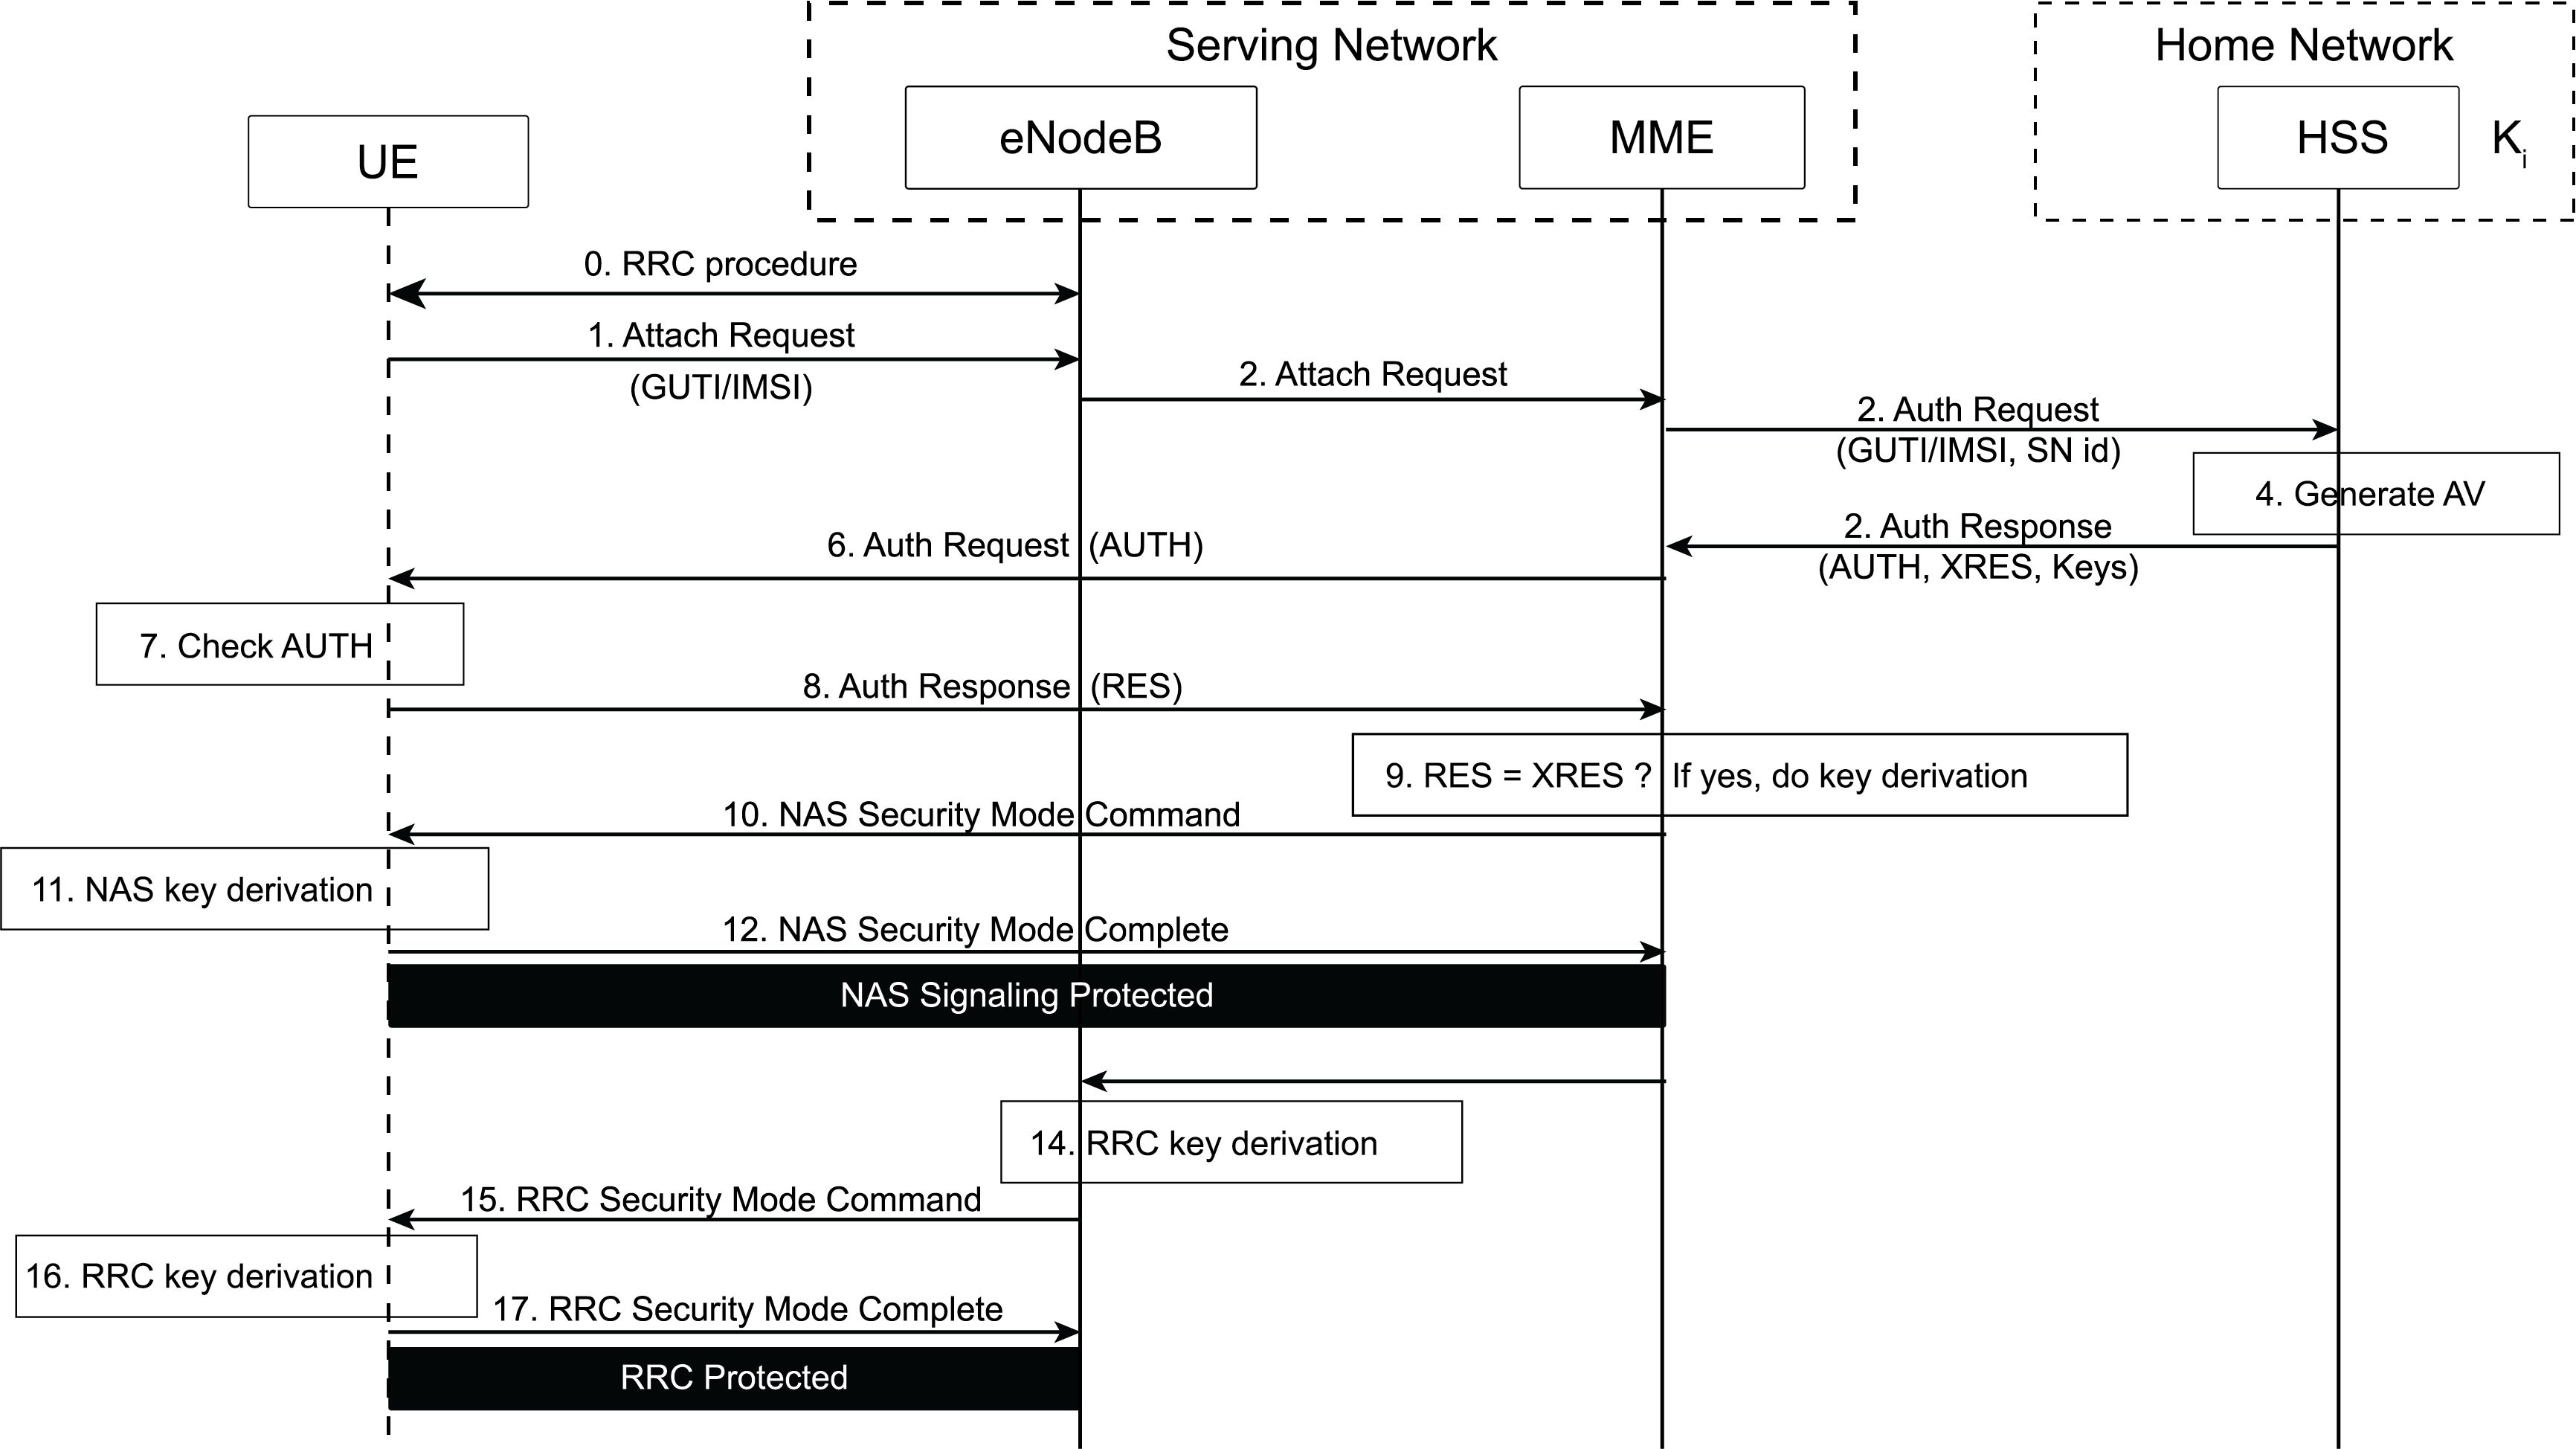
\includegraphics[width=0.8\textwidth]{figs/4g-authentication-flow.png}
    \caption{\ac{4G} Authentication Procedure}
    \label{fig:single}
\end{figure}

\subsection{\acs{5G} Security Framework}

As mentioned before, \ac{5G} has a \acl{SBA}, and in this architecture, some of the new entities relevant to \ac{5G} authentication are:

\begin{itemize}
    \item{
        The \ac{SEAF}, which acts as a intermidiary between the \ac{UE} and its home network, during the authentication process. It has the capability to out right reject and \ac{UE} but is dependent on the \ac{HN} to validate the authentication.
    }
    \item{
        The \ac{AUSF} is responsible to deciding if the \ac{UE} get authenticated.
    }
    \item{
        The \ac{UDM} hosts the \ac{ARPF}, responsible for selecting the authentication method, based on the subscribet identity and configured policy. It will also compute the authentication data for \ac{AUSF}.
    }
    \item{
        The \ac{SIDF} will be responsible for obtaining the \ac{SUPI} by decrypting the \ac{SUCI}.
    }
\end{itemize}

One of the main goals for \ac{5G} was the unification of authentication by making it open and access-network agnostic. In order to make it open, \ac{5G} rellies havily on \ac{EAP}, and when used the authentication will take place between the \ac{UE}, acting as the supplicant, the \ac{AUSF}, acting has the authenticaion server, through the \ac{SEAF} acting as an authenticator~\cite{rfc3748}.

Each generation of cellular networks has defined at least one new authentication method. For example, \ac{4G} introduced \ac{EPS-AKA}, and \ac{5G} introduced three authentication methods: \ac{5G-AKA}, \ac{EAP-AKA'}, and \ac{EAP-TLS}.

\subsection{Comparing \acs{5G-AKA}, \ac{EAP-AKA'} and \ac{EAP-TLS}}

The process begins when the \ac{SEAF} initiates authentication after receiving a message from the \ac{UE}. The \ac{UE} provides either a \ac{5G-GUTI} or a \ac{SUCI}.

The \ac{AUSF} first verifies that the requesting network is authorized. It then sends an authentication request to \ac{UDM}/\ac{ARPF}. If the \ac{SUCI} is provided, it's decrypted by the \ac{SIDF} to retrieve the \ac{SUPI}, which is then used to select the authentication method. \ac{UDM}/\ac{ARPF} generates an authentication response that includes tokens and keys, which are used by the \ac{AUSF} to compute a hash (\ac{HXRES}) and verify the expected response.

The \ac{AUSF} sends the authentication response to the \ac{SEAF} with the \ac{AUTH} token and \ac{HXRES}. At this point, the \ac{SUPI} is still not shared with the \ac{SEAF}. The \ac{SEAF} then forwards the \ac{AUTH} token to the \ac{UE}, which validates it using a secret key shared with the home network. If successful, the \ac{UE} computes and sends a response (\ac{RES} token) back to the \ac{SEAF}. The \ac{SEAF} validates this and forwards it to the \ac{AUSF} for final validation.

Once the \ac{RES} token is verified by the \ac{AUSF}, it sends an anchor key to the \ac{SEAF}, which then derives an \ac{AMF} key. The \ac{AMF} uses this key to generate further keys for protecting signaling messages between the \ac{UE} and the network elements. The \ac{UE}, with its root key, can derive all necessary keys for secure communication with the network, ensuring a shared and secure set of keys between the \ac{UE} and the network.

\ac{EAP-AKA'} is an alternative authentication method in \ac{5G}, providing mutual authentication between the \ac{UE} and the network based on a shared cryptographic key. Like \ac{5G-AKA}, it ensures strong security properties but has different message flows since it is based on \ac{EAP}. In this method, \ac{EAP} messages are encapsulated in \ac{NAS} messages between the \ac{UE} and the \ac{SEAF}, and in \ac{5G} service messages between the \ac{SEAF} and the \ac{AUSF}. In \ac{EAP-AKA'}, the \ac{SEAF} acts as a transparent relay, forwarding \ac{EAP} messages between the \ac{UE} and the \ac{AUSF} without participating in authentication decisions. In contrast, in \ac{5G-AKA}, the \ac{SEAF} verifies the \ac{UE}'s authentication response and can act on failures. Also, in 5G-AKA, the \ac{KAUSF} is computed by \ac{UDM}/\ac{ARPF} and sent to the \ac{AUSF} while in \ac{EAP-AKA'}, the \ac{AUSF} derives the \ac{KAUSF} from keying materials provided by the \ac{UDM}/\ac{ARPF}, using an \ac{EMSK} as specified in \ac{EAP}.

Lastly we have \ac{EAP-TLS} which is a subscriber authentication method in \ac{5G}, designed for specific scenarios like private networks and \ac{IoT}. When selected by \ac{UDM}/\ac{ARPF}, \ac{EAP-TLS} operates between the \ac{UE} and the \ac{AUSF} through the \ac{SEAF}, which acts as a transparent \ac{EAP} authenticator, forwarding \ac{EAP-TLS} messages. With \ac{EAP-TLS} we still achieve mutual authenticaion, this time via verification of public key certificates or a pre-shared key (\ac{PSK}) established through \ac{TLS} handshakes or out-of-band methods.

Some fundamental differences between this method and the previous AKA-based ones include the trust model: in \ac{EAP-TLS}, mutual trust is based on public key certificates, unlike AKA methods, which rely on symmetric keys shared between the \ac{UE} and the network. Additionally, \ac{EAP-TLS} eliminates the need to store numerous long-term symmetric keys in the home network (\ac{UDM}), reducing risks in key management. Another key difference that makes \ac{EAP-TLS} extremely well-suited for our use case is that it does not require the \ac{UE} to have a \ac{USIM}~\cite{cbl-comp-4g-5g-p12}.

\subsection{What is \ac{3GPP} and non-\ac{3GPP} access?}

ac{3GPP} encompasses standards for mobile networks like \ac{3G}, \ac{4G}, and \ac{5G}, which are cellular technologies enabling network services from mobile carriers. In contrast, non-\ac{3GPP} refers to access technologies not standardized by \ac{3GPP}, such as Wi-Fi or satellite networks, which can still integrate with \ac{3GPP} networks but follow different standards (e.g., IEEE for Wi-Fi).

Within \ac{3GPP} architecture, the terms trusted and untrusted define how non-\ac{3GPP} networks connect to the mobile core. Trusted networks are verified and approved by the mobile operator, connecting directly to the core network using secure protocols, similar to \ac{3GPP} networks. For instance, a mobile operator’s managed Wi-Fi network may be trusted. On the other hand, untrusted networks, like public Wi-Fi hotspots managed by third parties, do not meet these standards and are treated differently.

\section{Wi-Fi Integration Challenges}

\section{Authentication and Identity Management in \acs{5G}}

% subsection:
%   - What is a GUTI, SUPI, SUCI and NAI?

\section{Current Solutions and Proposals}
\chapter{Methodology And Proposed Framework}%
\label{chapter:methodology-and-proposed-framework}

\begin{introduction}
This chapter explains the research approach undertaken to tackle challenges of integrating \ac{NAUN3} devices into \ac{5G} networks. Outlines the specific methodologies employed for analysis of compatible authentication mechanisms as well as for managing device identity. Furthermore, it presents the designed framework for seamless, secure integration, detailing the motivation behind the architecture as well as essential building blocks.
\end{introduction}

\section{Overall Research Approach}

This research followed a constructivist methodology to develop a novel solution for integrating \ac{NAUN3} devices into \ac{5G} networks by repurposing existing \ac{5G} facilities and capabilities.

The initial phase involved a detailed study of the \ac{5G} architecture and relevant \ac{3GPP} standards. Although these standards include mechanisms for non-\ac{3GPP} access and for managing devices behind residential \acp{5G-RG}, they fall short of addressing the specific challenges posed by \ac{NAUN3} devices—particularly in terms of \ac{USIM} requirements and the inability to perform standard \ac{5G} authentication. The core issue identified was enabling \ac{5GC} acceptance, indirect authentication, and per-device handling without requiring changes to either the \ac{NAUN3} devices or the \ac{5GC} itself. Concepts such as \acp{CGID}~\cite{23.316-p27} and \ac{PDU} session separation were explored for inspiration, although detailed implementation strategies for such contexts are not specified in current standards.

To minimize required changes to both the \ac{5GC} and \ac{NAUN3} devices, the proposed solution centers on implementing all adaptation logic within the \ac{5G-RG}. This approach ensures transparency to both the core network and the end devices, while granting control to the network operator.

The central methodology involved designing a framework in which the \ac{5G-RG} acts as a mediator. This framework employs local authentication (specifically \ac{EAP-TLS}), with the \ac{5G-RG} serving as an authenticator that forwards requests to a mandatory, operator-controlled external \ac{EAP} server. This server authenticates devices lacking native \ac{5G} identities. Upon successful local authentication, the \ac{5G-RG} establishes a dedicated \ac{PDU} Session in the \ac{5GC} for each authenticated device. This session acts as a 'proxy identity', allowing the \ac{5GC} to manage the device's traffic without requiring direct knowledge of its non-\ac{5G} credentials. The \ac{5G-RG} also handles traffic forwarding between the device and its associated \ac{PDU} Session.

This framework, designed to meet integration requirements with minimal disruption, was subsequently detailed, prototyped in a testbed, and validated through functional and security testing, as elaborated in the following chapters. The approach was selected for its potential to deliver a practical, minimally invasive solution to the integration challenge.

\section{Requirements Analysis}

To address the challenge of integrating \ac{NAUN3} devices lacking native \ac{5G} credentials, while maintaining minimal disruption to existing systems, the following key requirements were defined to guide the framework design:

\begin{enumerate}
    \item {
        \textbf{Minimal Impact on Existing Infrastructure}
        \begin{enumerate}
            \item {
                \textbf{Core Network:} Standard \acl{5GC} functions (\acl{AMF}, \acl{SMF}, \acl{UPF}) must remain unaltered at the code level, with only configuration changes (e.g., \ac{IP} bindings, \ac{DNN} definitions) permitted.
            }
            \item {
                \textbf{End Devices:} \ac{NAUN3} devices must operate without hardware or software modifications, requiring only standard \ac{EAP} Supplicant functionality.
            }
            \item {
                \textbf{\acl{RAN}:} Standard \ac{5G} \ac{RAN} components (\acp{gNB}) must function without modification, maintaining standard interface operations with the core.
            }
        \end{enumerate}
    }
    \item {
        \textbf{\ac{5G-RG}-Centric Intelligence}
        \begin{itemize}
            \item {
                All adaptation logic must reside within the network's \ac{5G-RG}, which mediates between the \ac{NAUN3} device and the \ac{5GC}, in support of the minimal-impact goal.
            }
        \end{itemize}
    }
    \item {
        \textbf{Functional Requirements}
        \begin{itemize}
            \item {
                \textbf{Secure Device Onboarding:} Devices must be locally authenticated via \ac{EAP-TLS}, with the \ac{5G-RG} relaying requests to an operator-controlled external \ac{EAP} server.
            }
            \item {
                \textbf{Individual Device Representation:} Each authenticated device must be assigned a unique \ac{PDU} Session within the \ac{5GC}, serving as a proxy identity.
            }
            \item {
                \textbf{Traffic Separation:} Internal service traffic (e.g., \ac{RADIUS} communication) and end-device traffic must be clearly separated within the \ac{5G} transport network.
            }
            \item {
                \textbf{Lifecycle Management:} The \ac{5G-RG} must manage each device's session from initial authentication to disconnection, including re-authentication and \ac{PDU} Session teardown.
            }
            \item {
                \textbf{Traffic Mapping and Isolation:} The \ac{5G-RG} must ensure precise mapping and isolation of traffic between each device and its dedicated \ac{PDU} Session.
            }
        \end{itemize}
    }
    \item {
        \textbf{Operational Requirements}
        \begin{enumerate}
            \item {
                \textbf{Transparency:} The system must appear standard to both the \ac{5GC} (via \ac{PDU} procedures) and the \ac{NAUN3} device (via \ac{EAP} authentication).
            }
            \item {
                \textbf{Operator Manageability:} The complete solution, including \ac{5G-RG} logic and external \ac{EAP} infrastructure, must be operator-deployable and manageable.
            }
        \end{enumerate}
    }
\end{enumerate}

Together, these requirements establish the foundation for a solution that integrates unmodified \ac{NAUN3} devices into the \ac{5G} ecosystem with minimal disruption to existing network components and processes.


\section{Proposed Authentication Mechanism}

To securely onboard \ac{NAUN3} devices lacking native \ac{5G} credentials, this framework employs \ac{EAP-TLS}—a mutual certificate-based authentication method offering strong security and compatibility with standard operator-managed components like \ac{RADIUS} servers. \ac{EAP-TLS} is particularly suitable for \ac{IoT} devices, where password-based methods are often impractical or insecure.

\begin{figure}
    \centering
    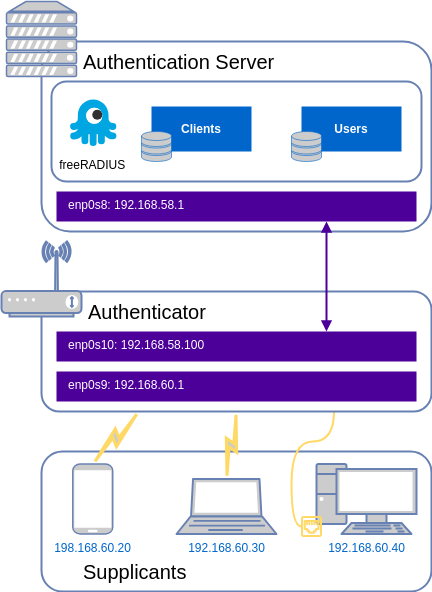
\includegraphics[width=0.5\linewidth]{figs/topology-EAP.png}
    \caption{\ac{EAP-TLS} Topology}
    \label{fig:EAP-TLS-topology}
\end{figure}

Figure~\ref{fig:EAP-TLS-topology} illustrates the architecture, which comprises three roles:

\begin{enumerate}
    \item {
        \textbf{Supplicant (NAUN3 Device):} Initiates the authentication using client-side \ac{EAP-TLS} and must be pre-provisioned with:
        \begin{itemize}
            \item A unique identity (e.g., username or \ac{MAC} address)
            \item A \ac{CA} certificate to validate the server
            \item A client certificate and private key (optionally password-protected)
        \end{itemize}
        Standard software such as \texttt{wpa\_Supplicant} is used to handle this role.
    }
    \item {
        \textbf{Authenticator (5G-RG):} Acts as a relay, not terminating the \ac{EAP-TLS} session. Responsibilities include:
        \begin{itemize}
            \item Detecting device connection attempts
            \item Initiating the \ac{EAP} exchange (e.g., via \texttt{hostapd})
            \item Relaying \ac{EAP} messages over \ac{RADIUS} through the \texttt{backhaul} \ac{DNN}
            \item Maintaining device authentication states
            \item Triggering \ac{PDU} Session establishment upon successful authentication
        \end{itemize}
    }
    \item {
        \textbf{Authentication Server (e.g., FreeRADIUS):} Typically managed by the same \ac{ISP} operating the \ac{5GC}. Its functions are:
        \begin{itemize}
            \item Managing identities and issuing credentials
            \item Terminating and validating the \ac{EAP-TLS} session
            \item Authenticating clients via certificate verification
            \item Returning \ac{EAP}-Success or \ac{EAP}-Failure via \ac{RADIUS}
        \end{itemize}
    }
\end{enumerate}

\begin{figure}
    \centering
    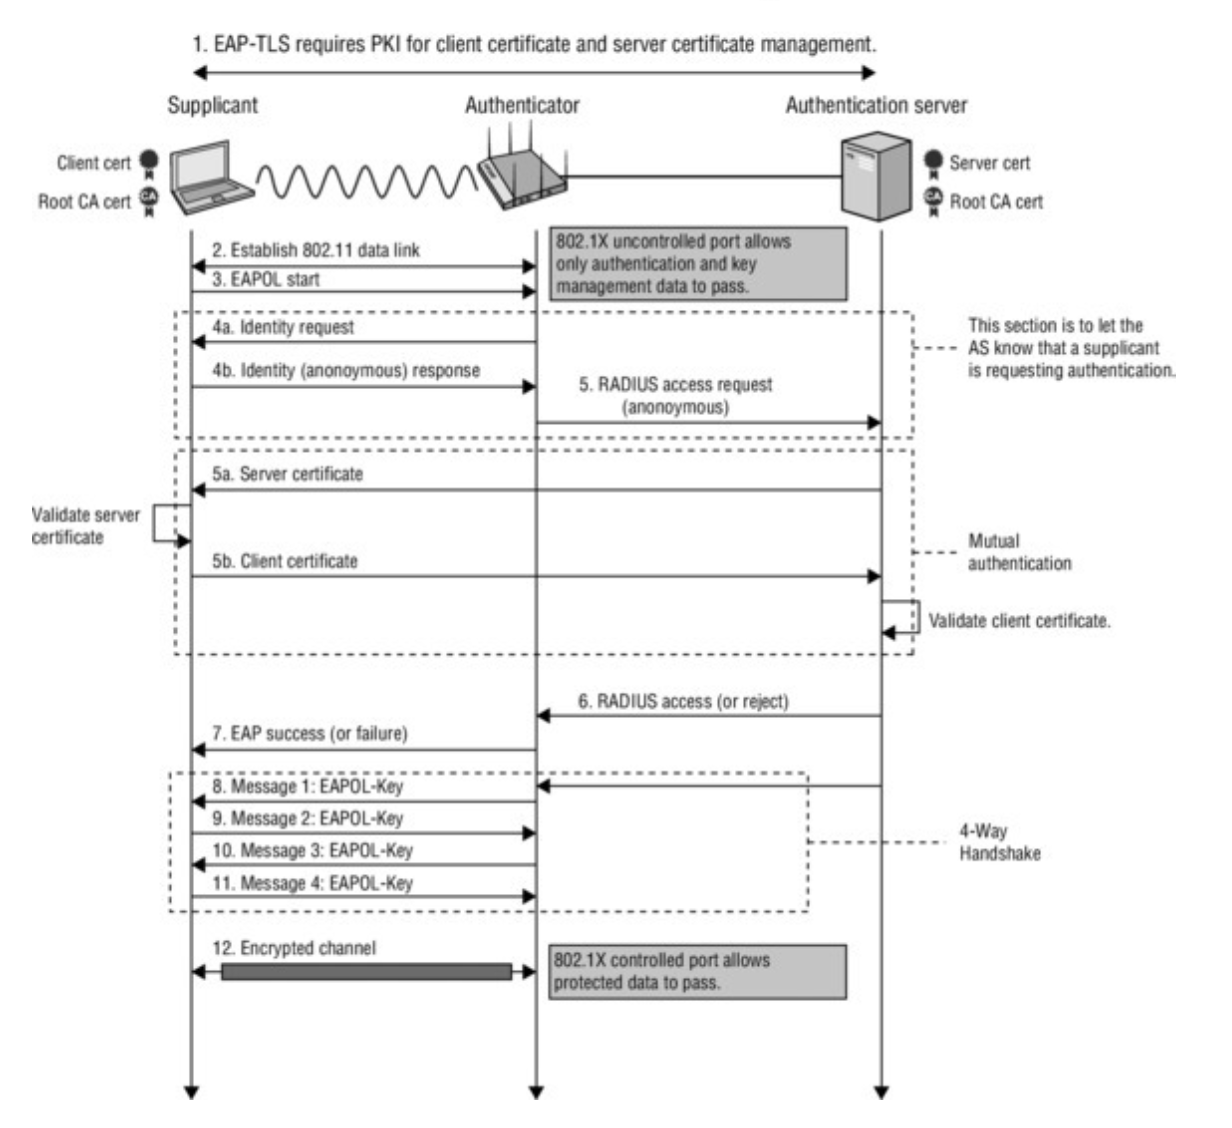
\includegraphics[width=0.75\linewidth]{figs/eap-tls-auth-flow.png}
    \caption{\ac{EAP-TLS} Authentication Flow}
    \label{fig:eap-tls-auth-flow}
\end{figure}

The \ac{EAP-TLS} authentication procedure, shown in Figure~\ref{fig:eap-tls-auth-flow}, follows these steps:

\begin{enumerate}
    \item Supplicant establishes a link-layer connection with the \ac{5G-RG} (e.g., via Wi-Fi or Ethernet).
    \item It sends an \ac{EAPOL}-Start to initiate authentication.
    \item The 5G-RG replies with an \ac{EAP}-Request/Identity.
    \item The Supplicant responds with an \ac{EAP}-Response/Identity (potentially anonymous).
    \item The 5G-RG relays this via a \ac{RADIUS} Access-Request to the Authentication Server.
    \item The server replies with its certificate inside an \ac{EAP}-Request (via Access-Challenge).
    \item The Supplicant validates the server certificate using its \ac{CA}.
    \item The client certificate is returned via \ac{EAP}-Response (also through Access-Challenge).
    \item Mutual authentication is completed when the server verifies the client certificate.
    \item The server sends \ac{RADIUS} Access-Accept with \ac{EAP}-Success (or Access-Reject with \ac{EAP}-Failure).
    \item The 5G-RG relays the final \ac{EAP} result to the Supplicant.
    \item If successful, a secure link-layer connection is established (e.g., WPA2 4-Way Handshake).
\end{enumerate}

The \ac{5G-RG} interprets the final \ac{EAP} message as follows:

\begin{itemize}
    \item \textbf{\ac{EAP}-Success:} Triggers the 5G-RG to initiate a \ac{PDU} Session via the \texttt{clients} \ac{DNN}, binding the session to the authenticated device and handling traffic mapping.
    \item \textbf{\ac{EAP}-Failure:} Denies network access, terminating the process.
\end{itemize}

This mechanism assumes that devices are securely provisioned in advance with the required credentials. The provisioning process itself is considered out of scope for this implementation.

\section{Proposed Identity Management Solution}

\subsection{The Identity Management Challenge}

The deployment of Wi-Fi-only, or \ac{NAUN3}, devices in the \ac{5G} network poses a fundamental identity management problem. Standard \ac{5G} identification depends on the \ac{SUPI}, usually derived from credentials stored securely in a \ac{USIM} (such as an \ac{IMSI} or \ac{NAI}). The \ac{SUPI} over the air is encrypted as a \ac{SUCI}. Devices without a \ac{USIM} cannot create a \ac{SUPI} or \ac{SUCI}, and hence cannot be recognized, verified, or managed via standard \ac{5GC} processes.

\subsection{Core Concept: \ac{PDU} Sessions as Proxy Identities}

To remedy this, the solution takes advantage of the capabilities of the \ac{5G-RG} and the versatility of 5G session management. From the viewpoint of the \ac{5GC}, a \ac{5G-RG} will act like a regular \ac{UE}, including its own \ac{USIM}, credentials, and support for several simultaneous \ac{PDU} Sessions. This allows segregation of traffic for different services or endpoints.

Taking a cue from the idea of \acp{CGID}, in which \ac{PDU} Sessions might represent a set of devices behind a gateway (collectively by \acp{SSID} or by Ethernet ports), the solution suggests a finer-grained approach: allocating each successfully authenticated \ac{NAUN3} device its very own dedicated \ac{PDU} Session, and not aggregating them.

In the proposed model, every \ac{PDU} Session, created and owned by the \ac{5G-RG}, will be a proxy identifier of a particular device. This enables not just integration into the \ac{5GC}, but also the ability to define session-specific controls and policies, and thus personalized management.

\subsection{Establishing the Proxy Identity}

After a device has been successfully authenticated through \ac{EAP-TLS}, as described in the earlier section, the \ac{5G-RG} then initiates a \ac{PDU} Session Establishment procedure. This is done through its own credentials and \ac{SUPI}, to the \ac{SMF}, through the \ac{AMF}, and specifying the special-purpose \texttt{clients} \ac{DNN}.

Upon the assignment of resources — like an IP address — by the \ac{5GC} to the session, the session is bound by the \ac{5G-RG} to the authenticated \ac{NAUN3} device. From there on, the session becomes the device’s operational identity in the \ac{5G} system.

\subsection{Gateway’s Role in Identity Mapping}

The \ac{5G-RG} maintains an internal mapping table that links each \ac{NAUN3} device’s local identifier (e.g., \ac{MAC} address) to its associated \ac{PDU} Session ID. This mapping enables accurate routing of data between the local network and the corresponding session within the \ac{5GC}.

\subsection{\ac{5GC} Perspective and Management}

From the point of view of the \ac{5GC}, the procedure is all standard. It communicates to just one registered \ac{UE}, the \ac{5G-RG}, to establish and release numerous \ac{PDU} Sessions related to the \texttt{clients} \ac{DNN}. Each session is managed by the \ac{SMF}, and it follows traditional techniques for resource assignment, policy control, and life cycle management.

Specifically, the \ac{5GC} has no knowledge of the device identities or the authentication information of the end devices behind the \ac{5G-RG}, it merely controls the session at the request of the gateway.

\subsection{Lifecycle of the Identity Mapping}

The \ac{5G-RG} takes charge of the entire life-cycle of the proxy identity:

\begin{itemize}
    \item \textbf{Creation:} Upon successful \ac{EAP-TLS} authentication of an \ac{NAUN3} device, the gateway creates a mapping entry and asks the \ac{5GC} to create a dedicated
    
    \item \textbf{Maintenance:} The \ac{5G-RG} routes the device’s traffic through the corresponding \ac{PDU} Session and monitors the device’s local status (e.g., association state or heartbeat checks).

    \item {
        \textbf{Termination:} If the device disconnects or becomes inactive:
        \begin{enumerate}
            \item The gateway deauthenticates the device locally (e.g., via \texttt{hostapd}).
            \item It releases the associated \ac{PDU} Session via a standard release procedure to the \ac{5GC}.
            \item The internal mapping entry is removed.
        \end{enumerate}
    }
\end{itemize}

\subsection{Advantages of the Proposed Approach}

This session-based proxy identification scheme offers a number of beneficial features:

\begin{itemize}
    \item \textbf{Transparency:} The solution is transparent to both the \ac{NAUN3} device (which experiences usual local verification) and the \ac{5GC} (which maintains regular \ac{PDU} sessions).
    \item \textbf{Reuses Existing Infrastructure:} It constructs on top of existing \ac{5G} session management without the need to make any modifications to the core identity frameworks.

    \item \textbf{Localized Complexity:} Complexity of all sorts is centralized in the \ac{5G-RG}, reducing the need to integrate with
    
    \item \textbf{Fine-Grained Control:} End-device \ac{PDU} Sessions support per-device policy enforcement (i.e., traffic shaping or QoS) at the \ac{5GC}, providing fine-grained control
\end{itemize}

\section{Framework Architecture and Integration}

\subsection{Overall Architecture Overview}

\begin{figure}
    \centering
    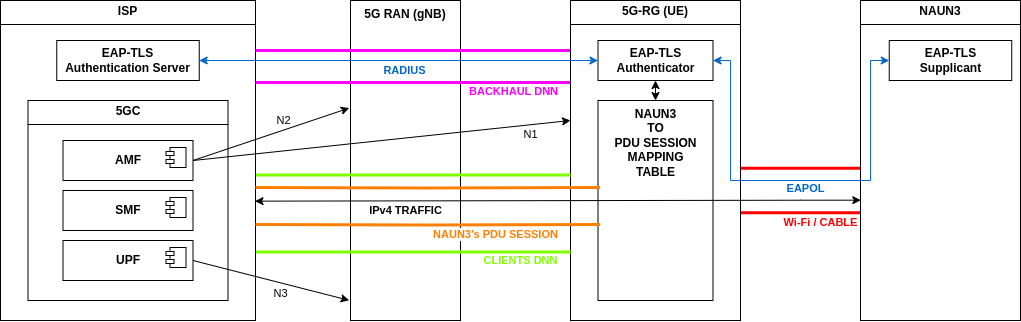
\includegraphics[width=0.75\linewidth]{figs/overall-topology.png}
    \caption{Overall Architecture}
    \label{fig:Overall Architecture}
\end{figure}

This top-level architecture Figure \ref{fig:Overall Architecture} shows the integration framework. The \ac{NAUN3} device connects locally (through Wi-Fi or cable) to the \ac{5G-RG}, the latter serving as a regular \ac{UE} to the \ac{5G} \ac{RAN} (\ac{gNB}) and to the \ac{5GC} (\ac{AMF}, \ac{SMF}, \ac{UPF}) and serving as an \ac{EAP} Authenticator forwarding requests to the external \ac{EAP-TLS} Authentication Server within the domain of the \ac{ISP}. The connection between the \ac{5G-RG} and the \ac{EAP} server is done through the use of \ac{RADIUS}, over a dedicated \ac{PDU} session belonging to the \texttt{backhaul} \ac{DNN}. Most importantly, when the local authentication of the \ac{5G-RG} was successful, the latter creates a different \ac{PDU} session for the \ac{NAUN3} device

\subsection{Key Communication Flows in the Integrated System}

\subsection{Interface and Protocol Integration}

A key aspect of this framework's design is its reliance on standard, well-defined interfaces and protocols, minimizing the need for proprietary extensions. The integration is achieved by orchestrating these standard elements in a specific manner, primarily through the logic implemented within the \ac{5G-RG}.

The main interfaces and protocols involved are:
\begin{itemize}
    \item {
        \textbf{Local Network Interface (between \ac{NAUN3} Device and the \ac{5G-RG}):}
        \begin{itemize}
            \item \textbf{Link Layer:} Standard Ethernet (\ac{IEEE} 802.3) or Wi-Fi (\ac{IEEE} 802.11).
            \item {Authentication:} Extensible Authentication Protocol over \ac{LAN} (\ac{EAPoL} - \ac{IEEE} 802.1X) is used to transport \ac{EAP} messages over the local link.
            \item \textbf{EAP Method:} \ac{EAP-TLS} is used for mutual authentication between the \ac{NAUN3} device (supplicant) and the \ac{EAP} infrastructure (via the \ac{5G-RG} relay).
        \end{itemize}
    }
    \item {
        \textbf{\ac{5G} Interfaces (between \ac{5G-RG} and the \ac{5GC}):}
        \begin{itemize}
            \item \textbf{N1 Interface:} Carries \ac{NAS} signaling between the \ac{5G-RG} and the \ac{AMF} for registration, authentication (of the \ac{RG} itself), and session management procedures.
            \item \textbf{N2 Interface:} Carries \ac{NGAP} signaling between the \ac{gNB}, which connects the \ac{5G-RG}, and the \ac{AMF}, primarily for \ac{UE} context management and \ac{PDU} session resource setup requests related to the \ac{5G-RG}.
            \item \textbf{N3 Interface:} Carries the user plane traffic encapsulated in \ac{GTP-U} tunnels between the \ac{gNB} and the \ac{UPF}. This includes traffic for both the \texttt{backhaul} \ac{PDU} session and all the individual \texttt{clients} \ac{PDU} sessions.
        \end{itemize}
    }
    \item {
        \textbf{Authentication Interface (between \ac{5G-RG} and the \ac{EAP} Authentication Server):}
        \begin{itemize}
            \item \textbf{Application Layer:} \ac{RADIUS} protocol is used to carry \ac{EAP} messages between the \ac{5G-RG} (acting as a \ac{RADIUS} client and \ac{EAP} authenticator) and the external authentication server).
            \item \textbf{Transport:} \ac{RADIUS} messages are transported over \ac{IP}, using \ac{UDP}. This \ac{IP} traffic is securely tunneled through the \ac{5G-RG}'s dedicated \texttt{backhaul} \ac{PDU} session via the \ac{N3} interface and \ac{UPF}.
        \end{itemize}
    }
\end{itemize}

The novelty lies not in modifying these protocols but in configuring the system components (\ac{5GC} \acp{NF}, \ac{5G-RG}, \ac{EAP} Server) and implementing the orchestration logic within the \ac{5G-RG} to manage the per-device proxy identity using standard \ac{5G} session management procedures.

\section{Scope and Assumptions}

This framework successfully brings \ac{NAUN3} devices into the \ac{5G} ecosystem by coordinating standard protocols and interfaces using smart logic centralized within the \ac{5G-RG}. Its main innovation is using individual \ac{PDU} Sessions, set up by the \ac{5G-RG}, as flexible proxy identities for each locally authenticated \ac{NAUN3} device. This method eliminates the need for devices to have native \ac{5G} credentials like \ac{SUPI} or \ac{USIM}.

Integration is handled dynamically across the device's connection lifecycle. After a device completes local \ac{EAP-TLS} authentication, the \ac{5G-RG} requests a dedicated \ac{PDU} Session (under the \texttt{clients} \ac{DNN}) from the \ac{5GC}. The \ac{5G-RG} keeps an internal mapping between the device's local identity and its assigned \ac{PDU} Session. If the device disconnects or loses connectivity, the \ac{5G-RG} promptly terminates the related \ac{PDU} Session to free up \ac{5G} resources, ensuring only active and authenticated devices consume network capacity.

Ultimately, this setup enables the \ac{5GC} to manage each device individually—applying policies like \ac{QoS} and routing—through standard \ac{PDU} Session management, all without requiring changes to the \ac{NAUN3} devices or \ac{5G} core network functions. Integration relies entirely on configurations and the gateway's mediation, avoiding any need to alter fundamental \ac{5G} protocols or the capabilities of the devices themselves.
\chapter{Development And Implementation}%
\label{chapter:development-and-implementation}

\begin{introduction}
Building upon the proposed framework, this chapter describes the practical development and implementation process undertaken. In this paper, the specific tools, technologies, and configurations used to realize the solution are described, including the construction of key modules and the configuration of the experimental environment required for subsequent validation.
\end{introduction}

\section{Development Environment and Tools}

To construct and validate the proposed framework, a virtualized multi-\ac{VM} environment was orchestrated using Vagrant with VirtualBox as the provider. This approach allowed for the creation of a reproducible and isolated network testbed. The environment consists of four distinct \acp{VM}, each running Ubuntu 22.04 LTS (Jammy Jellyfish) as the base operating system. The roles and typical resource allocations for these \acp{VM}, as defined in the \texttt{Vagrantfile}, are:

\begin{enumerate}
    \item \textbf{\texttt{core} \ac{VM}:} Hosts the \ac{5GC} functions and the \ac{EAP} Authentication Server. Allocated 2\ac{GB} \ac{RAM} and 1 \ac{CPU}.

    \item \textbf{\texttt{gnb} \ac{VM}:} Runs the \ac{gNB} simulator. Allocated 1\ac{GB} \ac{RAM} and 1 \ac{CPU}.

    \item \textbf{\texttt{ue} \ac{VM}:} Represents the \ac{5G-RG}, acting as a \ac{UE} towards the \ac{5GC} and as an \ac{EAP} Authenticator/Gateway towards the \ac{NAUN3} device. Allocated 1\ac{GB} \ac{RAM} and 1 \ac{CPU}.

    \item \textbf{\texttt{naun3} \ac{VM}:} Simulates the Wi-Fi-only/\ac{NAUN3} end device, acting as an \ac{EAP} Supplicant. Allocated 1\ac{GB} \ac{RAM} and 1 \ac{CPU}.
\end{enumerate}

The following core software components and tools were utilized across these \acp{VM}, installed and configured via shell scripts executed during Vagrant provisioning:

\begin{enumerate}
    \item  {
        \textbf{\ac{5G} Network Simulation:}
        \begin{itemize}
            \item \textbf{Open5GS:} The open-source implementation of \ac{5GC} functions (\ac{AMF}, \ac{SMF}, \ac{UPF}, \ac{NRF}, \ac{AUSF}, \ac{UDM}, \ac{UDR}, \ac{PCF}, \ac{NSSF}). Installed on the \texttt{core} \ac{VM}.

            \item \textbf{MongoDB:} Used as the database backend for Open5GS, storing subscriber information and network function configurations. Installed from the official MongoDB repositories on the \texttt{core} \ac{VM}.

            \item \textbf{UERANSIM:} An open-source \ac{gNB} and \ac{UE} simulator. Cloned from its GitHub repository and compiled from source on the \texttt{gnb} \ac{VM} (for \ac{gNB} functionality) and the \texttt{ue} \ac{VM} (for \ac{UE}/\ac{5G-RG} functionality). The \texttt{nr-cli} utility from UERANSIM was also made available
        \end{itemize}
    }

    \item {
        \textbf{Authentication Infrastructure:}
        \begin{itemize}
            \item \textbf{FreeRADIUS:} Employed as the \ac{EAP-TLS} Authentication Server. Installed on the \texttt{core} \ac{VM} and configured to handle \ac{EAP-TLS}, manage client (\ac{UE}/\ac{5G-RG}) definitions, and generate/use X.509 certificates.

            \item \textbf{\texttt{hostapd}:} Utilized as the \ac{EAP} Authenticator on the \texttt{ue} \ac{VM} (\ac{5G-RG}). Cloned from its official repository (\texttt{w1.fi/hostap.git}) and compiled from source with the \texttt{CONFIG\_DRIVER\_WIRED=y} option enabled to support \ac{EAP} over wired interfaces for the \ac{NAUN3} device connection.

            \item \textbf{\texttt{wpa\_supplicant}:} Used as the \ac{EAP} Supplicant on the \texttt{naun3} \ac{VM}. Installed via \texttt{apt} and configured to perform \ac{EAP-TLS} authentication using client certificates.
        \end{itemize}
    }

    \item {
        \textbf{Networking and Utility Tools:}
        \begin{itemize}
            \item \textbf{\texttt{dnsmasq}:} Configured as a \ac{DHCP} server on the \texttt{ue} \ac{VM} to provide \ac{IP} addresses to \ac{NAUN3} devices connecting to its local network interface (\texttt{enp0s9}).

            \item \textbf{\texttt{yq}:} A command-line YAML processor, installed via \texttt{snap}. Extensively used in provisioning scripts to modify Open5GS and UERANSIM configuration files (e.g., setting \ac{IP} addresses, \acp{DNN}, \acp{APN}).

            \item \textbf{Build Tools:} \texttt{make}, \texttt{git}, \texttt{gcc}, \texttt{g++}, \texttt{cmake} (via \texttt{snap}), \texttt{libsctp-dev}, \texttt{lksctp-tools}, \texttt{pkgconf}, \texttt{libssl-dev}, \texttt{libnl-3-dev}, \texttt{libnl-genl-3-dev} were installed for compiling UERANSIM and \texttt{hostapd} from source.

            \item \textbf{System Utilities:} \texttt{iproute2}, \texttt{net-tools}, \texttt{curl}, \texttt{gnupg} were used for network configuration and repository management.

            \item \textbf{Node.js and Nginx:} Installed on the \texttt{core} \ac{VM} to support and expose the Open5GS WebUI.
        \end{itemize}
    }

    \item {
        \textbf{Custom Tools and Scripts}
        \begin{itemize}
            \item \textbf{\texttt{open5gs-dbctl}:} A shell script provided and used on the \texttt{core} VM to interact with the MongoDB database for managing Open5GS subscriber entries (adding \acp{UE}, defining \acp{APN} and slices).

            \item \textbf{\texttt{interceptor}:} A custom Go application (compiled from source located in an \texttt{interceptor} directory, as indicated in the \texttt{Vagrantfile}) deployed on the \texttt{ue} \ac{VM}. This is the key tool developed to orchestrate the logic for monitoring \texttt{hostapd} events and managing \ac{PDU} sessions. It's specific internal workings are detailed later.

            \item \textbf{Provisioning Scripts:} A set of shell scripts (\texttt{core\_install}, \texttt{gnb\_install}, \texttt{ue\_install}, \texttt{naun3\_install}, \texttt{auth\_server\_install}, \texttt{ueransim\_install}) were used by Vagrant to automate the installation and configuration of all software components on their respective \acp{VM}.
        \end{itemize}
    }
\end{enumerate}

\subsection{Network Topology and Configuration Management}

The \texttt{Vagrantfile} defines several private networks to interconnect the \acp{VM}, establishing distinct network segments for communication between the \ac{5GC} and \ac{gNB} (\texttt{192.168.56.0/24}), \texttt{gNB} and \ac{UE}/\ac{5G-RG} (\texttt{192.168.57.0/24}), and the \ac{UE}/\ac{5G-RG}'s local network for \ac{NAUN3} devices (\texttt{192.168.60.0/24}). \ac{IP} addresses for various interfaces and services (e.g., \texttt{CORE\_IP}, \texttt{GNB\_IP\_CORE}, \texttt{UE\_LAN\_IP}, \texttt{AUTH\_SERVER\_IP} for \ac{RADIUS} communication over the \texttt{backhaul} tunnel) are explicitly defined and passed as arguments to the provisioning scripts.

Vagrant's synced folder feature was utilized to share:

\begin{itemize}
    \item \ac{EAP}/\ac{RADIUS} certificates generated by FreeRADIUS on the \texttt{core} \ac{VM} to the \texttt{naun3} \ac{VM} (via \texttt{/certs} on the guest).

    \item Runtime logs from all \acp{VM} to a \texttt{./build/runtime-logs} directory on the host machine.

    \item The compiled \texttt{interceptor} binary to the \texttt{ue} \ac{VM}.
\end{itemize}

This comprehensive setup provides a fully functional, albeit simulated, environment for developing and testing the proposed solution for integrating \ac{NAUN3} devices into a \ac{5G} network.

\section{Implementation of Proposed Authentication Logic}

% Detail how you implemented the specific EAP method or authentication flow defined in your methodology.

% Explain any code written for the device side (UE/Wi-Fi device simulator) and the network side (e.g., modifications to an EAP server, AUSF, or relevant gateway like W-AGF/TNGF).

\section{Implementation of Identity Management Mechanisms}

% Explain how you handle a device's unique identity withing the network

\section{Adaptation of Network Functions}

% Detail any modifications or specific configurations applied to simulated 5G core network functions (AMF, AUSF, UDM, potentially W-AGF/TNGF if simulating them separately).

% Explain how these functions were adapted to support the new authentication and identity schemes.

\section{System Integration and Configuration}

% Describe how the different implemented components (device, gateway, core network functions) were connected and configured to work together in your test environment.

% Include details about network configurations, interface setups, and parameter settings.

\section{Implementation Challenges}

% Briefly discuss any significant technical challenges encountered during development and how they were addressed.

\chapter{Validation and Results Evaluation}%
\label{chapter:validation-and-results-evaluation}

\begin{introduction}
This chapter presents the validation process and evaluates the performance and effectiveness of the implemented solution. Through a series of defined test scenarios and experiments, quantitative and qualitative results are gathered and analyzed. These findings are then critically assessed against the initial research objectives and compared with existing approaches discussed in the state of the art.
\end{introduction}

\section{Methodology}

To assess the feasibility, functionality, and effectiveness of the proposed solution, a series of tests were conducted within the simulated environment described in the \ref{chapter:development-and-implementation} chapter. The overall validation approach was simulation-based testing, leveraging the orchestrated virtual machines and configured \ac{5G} components (Open5GS, UERANSIM) and local network services (\texttt{hostapd}, \texttt{dnsmasq}, and the custom \texttt{interceptor} application).

The validation focused on several key aspects of the system:

\subsection{Overall Validation Approach}

\begin{itemize}
    \item \textbf{Simulation-Based Testing:} All validation activities were performed within the virtualized environment created using Vagrant, Open5GS, UERANSIM, FreeRADIUS, and the custom \texttt{interceptor} application. This allowed for controlled and repeatable testing of the end-to-end solution.

    \item \textbf{Focus on Functional Correctness and Integration:} The primary goal was to verify that the proposed mechanisms for authentication, proxy identity creation (per-device \ac{PDU} session), traffic mapping, and lifecycle management operate as designed.

    \item \textbf{Qualitative Security Assessment:} While not a formal security audit, the validation included observing whether the implemented security measures (\ac{EAP-TLS}, traffic separation) were functioning as intended.
\end{itemize}

\subsection{\acs{KPI}s and Metrics for Evaluation}

The evaluation of the framework centered on the following indicators and metrics, primarily assessed through functional testing and observation of system logs and behavior:

\begin{enumerate}
    \item{
        \textbf{Functional Correctness:}
        \begin{itemize}
            \item {
                \textbf{\ac{NAUN3} Device Authentication Success:}
                \begin{itemize}
                    \item \textbf{Metric:} Successful completion of the EAP-TLS authentication process for an NAUN3 device with the FreeRADIUS server, relayed by the 5G-RG (hostapd and interceptor).

                    \item \textbf{Verification:} Logs from \texttt{wpa\_supplicant} (\texttt{naun3} \ac{VM}), \texttt{hostapd} (\ac{5G-RG}/\texttt{ue} \ac{VM}), FreeRADIUS (\texttt{core} \ac{VM}), and the custom \texttt{interceptor} application on the \ac{5G-RG}. 
                \end{itemize}
            }
            \item {
                \textbf{Dedicated \ac{PDU} Session Establishment:}
                \begin{itemize}
                    \item \textbf{Metric:} Successful establishment of a unique \ac{PDU} session on the \texttt{clients} \ac{DNN} by the \ac{5G-RG} for each successfully authenticated \ac{NAUN3} device.

                    \item \textbf{Verification:} Output of \texttt{nr-cli ps-list} command on the \ac{5G-RG} (\texttt{ue} \ac{VM}); logs from Open5GS \ac{SMF} and \ac{UPF} on the \texttt{core} \ac{VM}. 
                \end{itemize}
            }
            \item {
                \textbf{\ac{IP} Address Allocation:}
                \begin{itemize}
                    \item \textbf{Metric (Local):} Successful assignment of a local \ac{IP} address to the \ac{NAUN3} device by \texttt{dnsmasq} on the \ac{5G-RG} after \ac{EAP-TLS} authentication.

                    \item \textbf{Metric (\ac{5GC}):} Successful assignment of a \ac{5GC} \ac{IP} address by the \ac{5GC} (\ac{SMF}/\ac{UPF}) to the dedicated \ac{PDU} session for the \ac{NAUN3} device.

                    \item \textbf{Verification:} \texttt{ip addr} command output on the \texttt{naun3} \ac{VM}; \texttt{dnsmasq} logs on the \ac{5G-RG}; \texttt{nr-cli ps-list} output on the \ac{5G-RG}; Open5GS \ac{SMF}/\ac{UPF} logs. 
                \end{itemize}
            }
            \item {
                \textbf{End-to-End Data Plane Connectivity:}
                \begin{itemize}
                    \item \textbf{Metric:} Ability of an authenticated \ac{NAUN3} device to send and receive \ac{IP} traffic to/from an external network via its dedicated \ac{PDU} session. 

                    \item \textbf{Verification:} Ping tests and simple data transfer from the \texttt{naun3} \ac{VM} to a target beyond the \ac{UPF}; packet captures (\texttt{tcpdump}) on \ac{NAUN3} \ac{LAN} interface, \ac{5G-RG}'s \ac{PDU} session tunnel interface, and \ac{UPF} interfaces.
                \end{itemize}
            }
            \item {
                \textbf{Traffic Isolation and Mapping:}
                \begin{itemize}
                    \item \textbf{Metric:} Confirmation that traffic from a specific \ac{NAUN3} device is routed exclusively through its dedicated \ac{PDU} session and associated routing rules. 

                    \item \textbf{Verification:} Packet captures on the \ac{5G-RG}; analysis of \texttt{iptables} counters, \texttt{ip rule} and \texttt{ip route} configurations on the \ac{5G-RG} during active traffic from one or more \ac{NAUN3} devices. 
                \end{itemize}
            }
            \item {
                \textbf{Lifecycle Management Correctness:}
                \begin{itemize}
                    \item \textbf{Metric:} Successful de-authentication of an \ac{NAUN3} device and termination of its associated \ac{PDU} session upon simulated disconnection/unreachability.

                    \item \textbf{Verification:} Logs from the \texttt{interceptor} application, \texttt{hostapd}, and \texttt{dnsmasq}; \texttt{nr-cli ps-list} output showing \ac{PDU} session release; verification of removal of \texttt{iptables} rules and \texttt{dnsmasq} permissions.
                \end{itemize}
            }
        \end{itemize}
    }
    \item{
        \textbf{Security Aspects (Qualitative Observation):}
        \begin{itemize}
            \item \textbf{\ac{EAP-TLS} Authentication Integrity:} Observation of the complete \ac{EAP-TLS} handshake and successful mutual authentication through detailed logs from involved components (\texttt{wpa\_supplicant}, \texttt{hostapd}, FreeRADIUS).

            \item \texttt{Traffic Segregation:} Confirmation via network monitoring and \ac{PDU} session analysis that \texttt{backhaul} \ac{DNN} traffic (e.g., \ac{RADIUS}) remains logically separate from the \texttt{clients} \ac{DNN} traffic (\ac{NAUN3} user plane data).

            \item \textbf{\ac{NAUN3} Identity Concealment from \ac{5GC}:} Verification that the \ac{NAUN3} device's local identifiers (e.g., \ac{MAC} address) are not directly signaled to or stored by the core \ac{5GC} \acp{NF} (\ac{AMF}, \ac{SMF}, \ac{UDM}), with the \ac{5G-RG} acting as the boundary.
        \end{itemize}
    }
    \item{
        \textbf{Resource Management (Observational):}
        \begin{itemize}
            \item \textbf{\ac{PDU} Session Correlation:} The number of active \ac{PDU} sessions on the \texttt{clients} \ac{DNN} should directly correspond to the number of currently authenticated and connected \ac{NAUN3} devices, as tracked by the \texttt{interceptor} application.

            \item \textbf{Timeliness of Operations (Qualitative):} General observation of the time taken for the end-to-end process: \ac{NAUN3} device \ac{EAP-TLS} authentication, subsequent \ac{PDU} session establishment, and the teardown process upon device disconnection. Formal latency measurements were considered outside the primary scope of this functional validation.
        \end{itemize}
    }
    \item{
        \textbf{System Stability and Robustness (Qualitative):}
        \begin{itemize}
            \item \textbf{Handling Multiple Devices:} The ability of the \texttt{interceptor} application and the overall simulated system to manage sequential and concurrent connections and disconnections of multiple \ac{NAUN3} devices without instability.

            \item \textbf{Error Handling:} Observation of error logging and any recovery mechanisms within the \texttt{interceptor} application in scenarios such as a failed \ac{PDU} session establishment attempt or unexpected disconnection.
        \end{itemize}
    }
\end{enumerate}

This validation methodology aims to provide a comprehensive assessment of the implemented solution's ability to meet its design goals, focusing on correct functionality and integration within the simulated \ac{5G} environment. The subsequent sections will detail the specific test scenarios designed and the evaluation of the results obtained.

\section{Test Scenarios and Setup}

To validate the different aspects of the proposed framework, a series of distinct test scenarios, or experiments, were designed and executed. These scenarios leveraged the fully configured simulation environment detailed in the \ref{chapter:development-and-implementation}, which includes the \texttt{core} \ac{VM} (Open5GS, FreeRADIUS), \texttt{gnb} \ac{VM} (UERANSIM gNB), \texttt{ue} \ac{VM} (5G-RG with UERANSIM UE, \texttt{hostapd}, \texttt{dnsmasq}, and the custom \texttt{interceptor} application), and one or more \texttt{naun3} \acp{VM} (\ac{EAP} supplicant).

Specific tools were employed for monitoring and verification in each scenario:

\begin{itemize}
    \item \textbf{Log Analysis:} Reviewing logs from Open5GS \acp{NF}, UERANSIM components, FreeRADIUS, \texttt{hostapd}, \texttt{wpa\_supplicant}, and the custom \texttt{interceptor} application was fundamental across all tests.

    \item \textbf{Packet Capture:} \texttt{tcpdump} and \texttt{tshark} (Wireshark \ac{CLI}) were used on various interfaces (\ac{NAUN3} \ac{LAN}, \ac{5G-RG}'s \texttt{backhaul} and \texttt{clients} \ac{PDU} session interfaces \texttt{uesimtunX}, \ac{gNB} interfaces) to inspect signaling and data plane traffic.

    \item \textbf{Network Utilities:} Standard Linux utilities like \texttt{ping} (with the \texttt{-R} record route option), \texttt{ip addr}, \texttt{ip route}, \texttt{ip rule}, \texttt{iptables -L -v -n -t mangle -t nat -t filter}, and UERANSIM's \texttt{nr-cli} were used for connectivity testing and state verification.

    \item \textbf{Traffic Generation and Throughput Measurement:} \texttt{iperf3} was used for generating controlled \ac{TCP}/\ac{UDP} network traffic between \ac{NAUN3} devices and a server on the \texttt{core} \ac{VM} (simulating an N6-connected server) to test data plane throughput and routing.

    \item \textbf{Timestamping/Scripting:} Basic shell scripting was used to capture timestamps before and after key events (e.g., `wpa\_supplicant` start and `dhclient` IP acquisition) to measure onboarding delay.
\end{itemize}

\subsection{Experiment 1: Single \acs{NAUN3} Device Onboarding and Basic Connectivity}

The objective was to verify the successful \ac{EAP-TLS} authentication of a single \ac{NAUN3} device, the subsequent establishment of its dedicated \ac{PDU} session on the \texttt{clients} \aDNN, local and 5GC IP address allocation, basic end-to-end data plane connectivity with path verification, and to measure the approximate onboarding delay.

Procedure:
\begin{enumerate}
    \item Ensure all \ac{5GC} \acp{NF}, \ac{gNB}, \ac{5G-RG} (including \texttt{hostapd} and \texttt{interceptor}), and FreeRADIUS are running. Start an \texttt{iperf3} server on the \texttt{core} \ac{VM} listening on the \ac{IP} address of its \texttt{clientun0} interface (e.g., \texttt{10.46.0.1}).

    \item On the \texttt{naun3} \ac{VM}, record a timestamp (\texttt{date +\%s}). Immediately start the \texttt{wpa\_supplicant} service.

    \item Monitor the authentication process through logs on the \texttt{naun3} \ac{VM}, \texttt{ue} \ac{VM} (\texttt{hostapd}, \texttt{interceptor}), and \texttt{core} \ac{VM} (FreeRADIUS).

    \item Once \texttt{wpa\_supplicant} indicates success and \texttt{dhclient} (run subsequently or as part of the script on \texttt{naun3}) obtains a local \ac{IP}, record another timestamp. Calculate the difference to estimate onboarding delay.
    
    \item Verify \ac{PDU} session establishment for the \texttt{clients} \ac{DNN} using \textttnr{-cli ps-list} on the \texttt{ue} \ac{VM}. Note the assigned \ac{5GC} \ac{IP} address for this \ac{PDU} session.
    
    \item Verify local \ac{IP} address assignment to the \texttt{naun3} \ac{VM} via \texttt{ip addr} on the \texttt{naun3} \ac{VM}.
    
    \item Verify the application of \texttt{iptables} and \texttt{ip rule}/\texttt{ip route} rules on the \texttt{ue} \ac{VM} specific to the authenticated \ac{NAUN3} device's \ac{MAC} and \ac{PDU} session ID.
    
    \item From the \texttt{naun3} \ac{VM}, initiate \texttt{ping -R <PDU\_Session\_Gateway\_IP>} (e.g., \texttt{10.46.0.1}). Analyze the recorded route to confirm it passes through the \ac{NAUN3}'s local \ac{IP}, then its assigned \ac{5GC} \ac{PDU} session \ac{IP}, and then to the target.
    
    \item From the \texttt{naun3} \ac{VM}, run an \texttt{iperf3} client connecting to the \texttt{iperf3} server on the \texttt{core} \ac{VM}.
    
    \item Capture traffic on relevant interfaces (\texttt{naun3} \ac{LAN}, \texttt{ue} \ac{VM} \ac{LAN}, \texttt{uesimtunX} on \texttt{ue} \ac{VM}, \texttt{clientun0} on \texttt{core} \ac{VM}) to observe data flow and \ac{NAT}.
\end{enumerate}

Metrics/Verification Points:
\begin{itemize}
    \item Successful \ac{EAP-TLS} authentication (logs).
    \item Onboarding delay (timestamp difference).
    \item One new \ac{PDU} session active on \texttt{clients} \ac{DNN} for the \ac{5G-RG}, with a unique \ac{5GC} \ac{IP}.
    \item \ac{NAUN3} device receives a local \ac{IP}.
    \item Successful \texttt{ping} with recorded route showing \ac{NAT} via the \ac{PDU} session IP.
    \item Successful \texttt{iperf3} data transfer.
    \item Correct \texttt{iptables} and policy routing rules applied.
\end{itemize}

\subsection{Experiment 2: Multi-Device Connectivity, Traffic Isolation, and \acs{PDU} Session Mapping}

In this experiment the goal was to verify that when multiple \ac{NAUN3} devices connect simultaneously, each gets a unique dedicated \ac{PDU} session, their traffic is correctly mapped and isolated, and \ac{NAT} occurs via their respective \ac{PDU} session \acp{IP}.

Procedure:
\begin{enumerate}
    \item Start two (or more) \texttt{naun3} \acp{VM} (e.g., \textt{naun301}, \texttt{naun302}), each configured with a client certificates for \ac{EAP-TLS}.

    \item Allow both devices to authenticate and establish their dedicated \ac{PDU} sessions as per Experiment 1. Verify that two distinct \texttt{clients} \ac{PDU} sessions are created by the \ac{5G-RG}, each with a unique \ac{5GC} \ac{IP} address (e.g., \texttt{10.46.0.3} and \texttt{10.46.0.4}).
    
    \item On the \texttt{ue} \ac{VM}, verify that distinct sets of \texttt{iptables} and \texttt{ip rule}/\texttt{ip route} entries are created for each \ac{NAUN3} device, mapping each to its unique \ac{PDU} session ID and tunnel interface.
    
    \item From \texttt{naun301}, execute \texttt{ping -R <PDU\_Session\_Gateway\_IP>}. Note the recorded route, particularly the \ac{5GC} \ac{IP} address assigned to \texttt{naun301}'s \ac{PDU} session.
    
    \item From \texttt{naun302}, execute \texttt{ping -R <PDU\_Session\_Gateway\_IP>}. Note the recorded route, verifying it uses a \textit{different} \ac{5GC} \ac{IP} address assigned to \texttt{naun302}'s \ac{PDU} session.
    
    \item Start an \texttt{iperf3} server on the \texttt{core} \ac{VM}.
    
    \item Simultaneously (or sequentially) run \texttt{iperf3} clients from \texttt{naun301} and \texttt{naun302} to the server on the \texttt{core} \ac{VM}.
    
    \item Monitor traffic on the \texttt{ue} \ac{VM}'s \texttt{uesimtunX} interfaces and check \texttt{iptables} counters to confirm traffic from each \ac{NAUN3} device is routed through its distinct \ac{PDU} session.
    
    \item On the \texttt{core} \ac{VM} (\texttt{iperf3} server logs), verify that connections are received from the distinct \ac{5GC} \ac{IP} addresses assigned to each \ac{NAUN3}'s \ac{PDU} session.
\end{enumerate}

Metrics/Verification Points:
\begin{itemize}
    \item Each \ac{NAUN3} device establishes its own unique \ac{PDU} session on the \texttt{clients} \ac{DNN} with a distinct \ac{5GC} \ac{IP}.
    
    \item \texttt{ping -R} from each \ac{NAUN3} shows a path \textit{NATted} through its unique \ac{PDU} session \ac{IP}.
    
    \item \texttt{iperf3} server logs show connections from distinct \ac{PDU} session \acp{IP}.
    
    \item \texttt{iptables} and routing rules correctly isolate traffic per device.
\end{itemize}

\subsection{Experiment 3: Lifecycle Management (Device Disconnection and Resource Cleanup)}

In order to verify that when an \ac{NAUN3} device disconnects or becomes unreachable, its local authentication is revoked, its dedicated \ac{PDU} session is terminated, and associated network resources (\ac{IP} addresses, routing rules) are correctly cleaned up by the \texttt{interceptor} the following procedure was followed.

\begin{enumerate}
    \item Successfully onboard a single \ac{NAUN3} device as per Experiment 1. Verify its \ac{PDU} session is active and traffic flows.

    \item{ Simulate device disconnection:
        \begin{itemize}
            \item \textbf{Option A (Graceful):} Stop the \texttt{wpa\_supplicant} service on the \texttt{naun3} \ac{VM}.
            \item \textbf{Option B (Abrupt):} Power off or disconnect the network interface of the \texttt{naun3} \ac{VM}.
        \end{itemize}
    }

    \item Monitor the \texttt{interceptor} logs on the \texttt{ue} \ac{VM} for detection of device unreachability and initiation of cleanup procedures.

    \item{
        Verify the following cleanup actions occur:
        \begin{itemize}
            \item \texttt{hostapd} deauthenticates the client (logs).

            \item The \texttt{interceptor} removes the device's \ac{MAC} from \texttt{/etc/allowed-macs.conf} and restarts \texttt{dnsmasq}.

            \item The \texttt{interceptor} removes the specific \texttt{iptables} and \texttt{ip rule}/\texttt{ip route} entries for the device.

            \item The \texttt{interceptor} initiates a \ac{PDU} session release for the \texttt{clients} \ac{DNN} using \texttt{nr-cli}.

            \item Verify using \texttt{nr-cli ps-list} that the \ac{PDU} session is terminated.
            
            \item Verify in Open5GS \ac{SMF}/\ac{UPF} logs that the session and associated resources are released.
        \end{itemize}
    }    
\end{enumerate}

Metrics/Verification Points:
\begin{itemize}
    \item Detection of device disconnection by the \texttt{interceptor}.
    \item Successful local deauthentication.
    \item Removal of \ac{DHCP} permission.
    \item Correct removal of all associated \texttt{iptables} and routing rules.
    \item Successful \ac{PDU} session termination in UERANSIM and Open5GS.
    \item Internal state of the \texttt{interceptor} (e.g., \texttt{allowedDevices} map) reflects the device removal.
\end{itemize}

\subsection{Experiment 4: Security Aspects Observation (Qualitative)}

To qualitatively observe key security aspects of the implemented solution, such as the \ac{EAP-TLS} handshake and traffic segregation, we performed the following:

\begin{enumerate}
    \item{
        During Experiment 1 (\ac{NAUN3} Device Onboarding):
        \begin{itemize}
            \item Use \texttt{tshark} or \texttt{tcpdump} on the \texttt{ue} \ac{VM}'s \ac{LAN} interface to capture the \ac{EAPOL} and \ac{EAP-TLS} handshake.

            \item Use \texttt{tshark} or \texttt{tcpdump} on the \texttt{ue} \ac{VM}'s \texttt{backhaul} \ac{PDU} session interface and on the \texttt{core} \ac{VM}'s interface connected to the \texttt{ue} \ac{VM}'s \texttt{backhaul} to capture \ac{RADIUS} traffic.
        \end{itemize}
    }
    \item{
        During Experiment 2 (Multiple Devices):
        \begin{itemize}
            \item Observe the source and destination \acp{IP} of the \ac{RADIUS} traffic on the \texttt{backhaul} \ac{PDU} session.
            
            \item Observe the source and destination \acp{IP} of the \ac{NAUN3} user plane traffic on the respective \texttt{clients} \ac{PDU} sessions.
        \end{itemize}
    }
\end{enumerate}

Metrics/Verification Points:
\begin{itemize}
    \item Observation of a complete and successful \ac{EAP-TLS} handshake.
    \item Confirmation that \ac{RADIUS} traffic is encapsulated and transported over the \texttt{backhaul} \ac{PDU} session.
    \item Confirmation that user plane traffic for each \ac{NAUN3} device is transported over its distinct \texttt{clients} \ac{PDU} session.
    \item Review of Open5GS logs (\ac{AMF}, \ac{SMF}) to confirm that only the \ac{5G-RG}'s identity (\ac{IMSI}) is used for \ac{5GC} signaling, and \ac{NAUN3} \ac{MAC} addresses are not propagated to these core \acp{NF}.
\end{itemize}

These experiments are designed to provide a holistic view of the system's functionality, its ability to manage multiple devices correctly, handle their lifecycle, and maintain basic security and traffic segregation principles, incorporating the specific types of data you've collected.

\section{Functional Validation Results}

This section presents the results obtained from executing the test scenarios described previously, demonstrating the functional correctness of the proposed authentication and identity management mechanisms. The evidence is drawn from system logs, network interface states, routing table configurations, and packet captures.

\subsection{\acs{NAUN3} Device Authentication and Onboarding:}
The primary test involved onboarding \ac{NAUN3} devices (\texttt{naun301}, \texttt{naun302}) one after another.

\begin{itemize}
    \item \textbf{EAP-TLS Authentication:} Logs from \texttt{wpa\_supplicant} on each \ac{NAUN3} device (see Listing \ref{lst:wpa_supplicant_eap_success}) confirmed the initiation and successful completion of the \ac{EAP-TLS} handshake ("\texttt{CTRL-EVENT-EAP-SUCCESS EAP authentication completed successfully}"). Correspondingly, the \texttt{hostapd} log on the 5G-RG (\texttt{ue} \ac{VM}) showed the \ac{EAP} exchange, including the relay of messages to the \ac{RADIUS} server and the reception of Access-Accept (see Listing \ref{lst:hostapd_naun301_eap_success}). The \texttt{interceptor} (see Figure \ref{fig:interceptor_eap_success}) captured the \texttt{CTRL-EVENT-EAP-SUCCESS} from \texttt{hostapd}, indicating its awareness of the successful local authentication.

    \begin{lstlisting}[caption=wpa\_supplicant successful authentication,label={lst:wpa_supplicant_eap_success}]
(...)
584| 1748702590.706948: enp0s8: CTRL-EVENT-EAP-SUCCESS EAP authentication completed successfully
585| 1748702590.706998: EAPOL: IEEE 802.1X for plaintext connection; no EAPOL-Key frames required
586| 1748702590.707047: enp0s8: WPA: EAPOL processing complete
587| 1748702590.707096: enp0s8: Cancelling authentication timeout
586| 1748702590.707147: enp0s8: State: ASSOCIATED -> COMPLETED
586| 1748702590.707201: enp0s8: CTRL-EVENT-CONNECTED - Connection to 01:80:c2:00:00:03 completed [id=0 id_str=]
(...)
    \end{lstlisting}

    \begin{lstlisting}[caption=\texttt{hostapd} successful authentication,label={lst:hostapd_naun301_eap_success}]
(...)
802| 1748702590.717640: EAP: EAP entering state SUCCESS2
803| 1748702590.717722: enp0s9: CTRL-EVENT-EAP-SUCCESS2 08:00:27:b4:18:a9
804| 1748702590.717775: CTRL_IFACE monitor send /tmp/interceptor_7025.sock\x00
805| 1748702590.717923: IEEE 802.1X: 08:00:27:b4:18:a9 BE_AUTH entering state SUCCESS
806| 1748702590.718200: 1748702590.718200: enp0s9: STA 08:00:27:b4:18:a9 IEEE 802.1X: Sending EAP Packet (identifier 224)
807| 1748702590.718452: IEEE 802.1X: 08:00:27:b4:18:a9 AUTH_PAE entering state AUTHENTICATED
808| 1748702590.718565: enp0s9: AP-STA-CONNECTED 08:00:27:b4:18:a9
(...)
    \end{lstlisting}

    \item{
        \textbf{Dedicated \ac{PDU} Session Establishment:} Following each successful \ac{EAP-TLS} authentication, the \texttt{interceptor} log shows the initiation of a new \ac{PDU} session request for the \texttt{clients} \ac{DNN} (see Figure \ref{fig:interceptor_eap_success}). The UERANSIM tool \texttt{nr-cli ps-list} on the \ac{5G-RG}, corroborates this (see Listing \ref{fig:ue_pdu_sessions}):
        \begin{itemize}
            \item Initially (14:43:09 \ac{UTC}), only \texttt{PDU Session1} (\ac{DNN}: \texttt{backhaul}, \ac{IP}: \texttt{10.45.0.2}) is active.
            
            \item After \texttt{naun301} (\ac{MAC} \texttt{08:00:27:b4:18:a9}) authenticates (around 14:43:10 \ac{UTC} in \texttt{interceptor} log), \texttt{PDU Session2} (\ac{DNN}: \texttt{clients}, \ac{IP}: \texttt{10.46.0.2}) becomes active by 14:43:30 \ac{UTC}.

            \item After \texttt{naun302} (\ac{MAC} \texttt{08:00:27:51:7f:ef}) authenticates (around 14:44:08 \ac{UTC} in \texttt{interceptor} log), \texttt{PDU Session3} (\ac{DNN}: \texttt{clients}, \ac{IP}: \texttt{10.46.0.3}) becomes active by 14:44:30 \ac{UTC}.
        \end{itemize}

        \begin{figure}
        \centering
            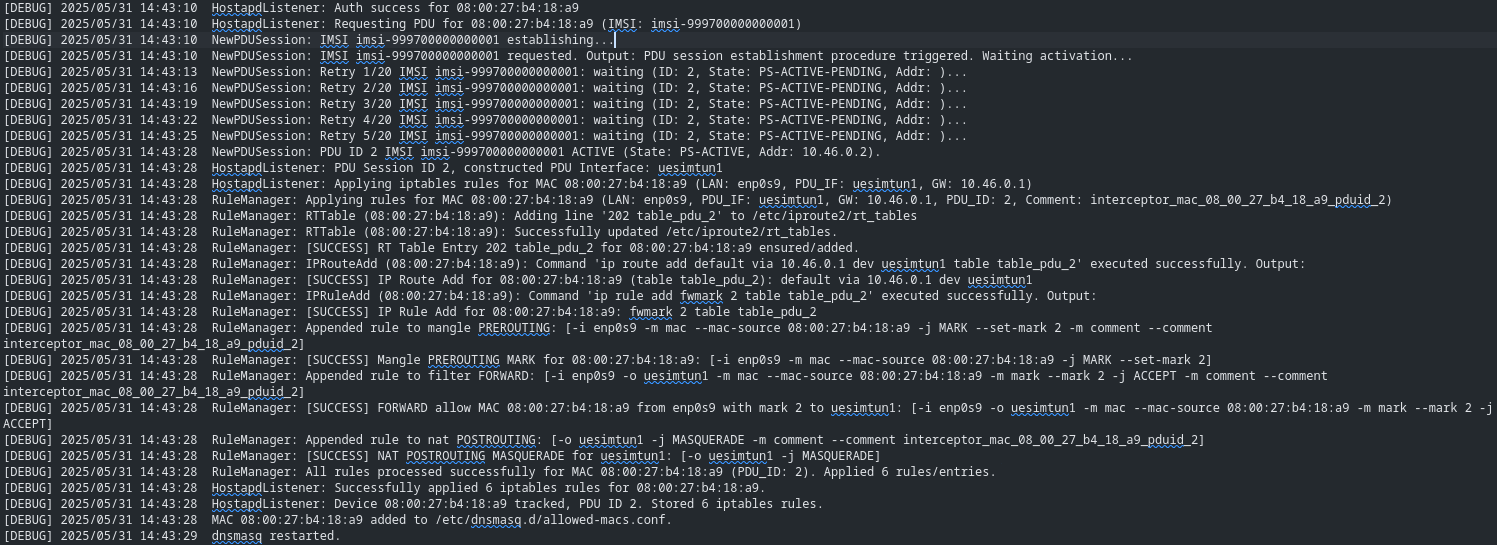
\includegraphics[width=1\linewidth]{figs/interceptor_eap_success.png}
            \caption{\texttt{interceptor} captures authentication success, requests \ac{PDU} session and applies mapping rules}
            \label{fig:interceptor_eap_success}
        \end{figure}

        \begin{figure}
            \centering
            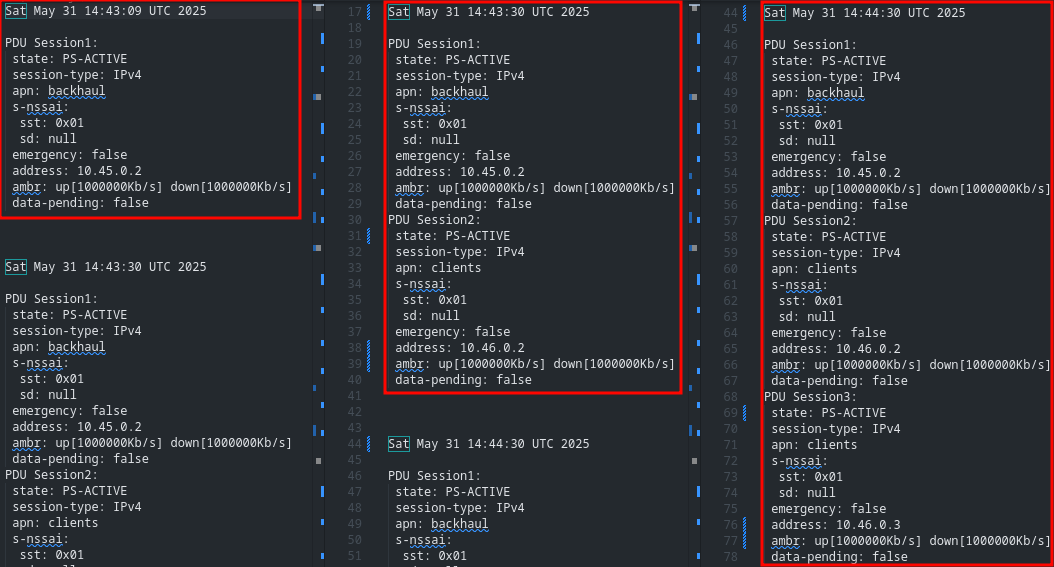
\includegraphics[width=1\linewidth]{figs/ue_pdu_sessions.png}
            \caption{\ac{PDU} Session via \texttt{nr-cli ps-list}}
            \label{fig:ue_pdu_sessions}
        \end{figure}
    }

    \item \textbf{Network Interface Creation:} The \texttt{ue} (see Figure \ref{fig:ue_pdu_sessions_nics}) log confirms the dynamic creation of network interfaces on the \ac{5G-RG} for each \texttt{clients} \ac{PDU} session. \texttt{uesimtun0} (\ac{IP} \texttt{10.45.0.2}) corresponds to the \texttt{backhaul} session. \texttt{uesimtun1} (\ac{IP} \texttt{10.46.0.2}) appears after \texttt{naun301} connects, and \texttt{uesimtun2} (\ac{IP} \texttt{10.46.0.3}) appears after \texttt{naun302} connects.

    \begin{figure}
        \centering
        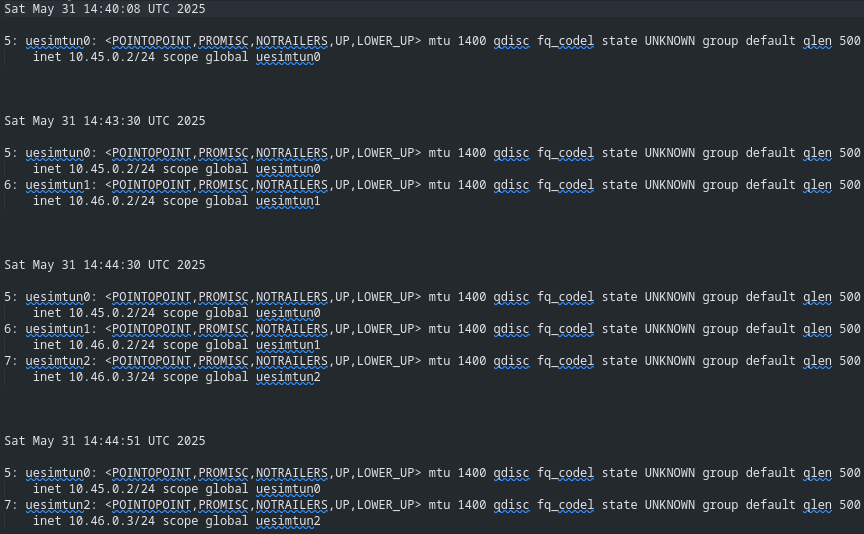
\includegraphics[width=1\linewidth]{figs/ue_pdu_sessions_nics.png}
        \caption{Network interfaces created by UERANSIM to bind to \ac{PDU} Sessions}
        \label{fig:ue_pdu_sessions_nics}
    \end{figure}

    \item \textbf{\ac{IP} Address Allocation:} The \ac{NAUN3} devices successfully obtained local \ac{IP} addresses from \texttt{dnsmasq} on the \ac{5G-RG} after authentication (see Figure \ref{fig:ping_gw}). The \ac{5GC} assigned unique \acp{IP} (\texttt{10.46.0.2}, \texttt{10.46.0.3}) to their respective \ac{PDU} sessions, as confirmed by Figures \ref{fig:ue_pdu_sessions} and \ref{fig:ue_pdu_sessions_nics}.

    \begin{figure}
        \centering
        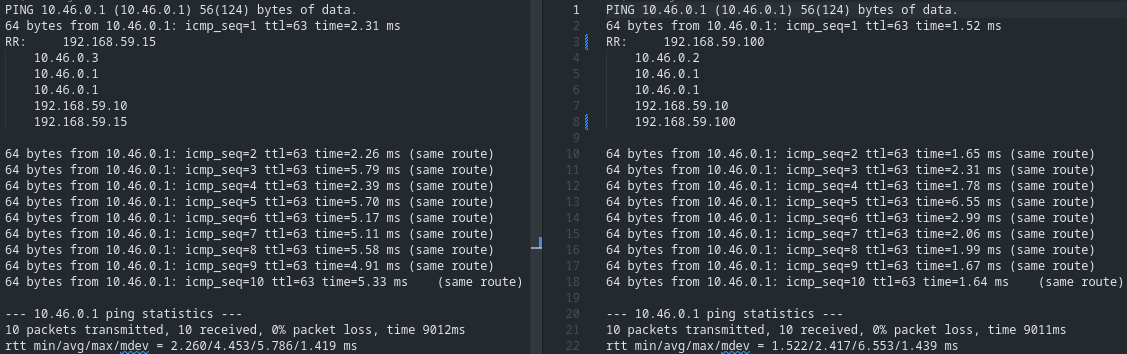
\includegraphics[width=1\linewidth]{figs/ping_gw.png}
        \caption{Pings from \texttt{naun301} and \texttt{naun302} to the \ac{5GC} gateway}
        \label{fig:ping_gw}
    \end{figure}
\end{itemize}

\subsection{End-to-End Connectivity and Path Verification}

Ping tests with the record route option (\texttt{-R}) were conducted from \texttt{naun301} and \texttt{naun302} (see Figure \ref{fig:ping_gw}) to the clients \ac{DNN} gateway \ac{IP} on the \texttt{core} \ac{VM} (\texttt{10.46.0.1}).

\begin{itemize}
    \item The recorded route when \texttt(naun301) pings the \ac{5GC} gateway is, \texttt{192.168.59.100} (\texttt{naun301} local \ac{IP}) -> \texttt{10.46.0.2} (\ac{PDU} Session 2 \ac{IP} for \texttt{naun302}) -> \texttt{10.46.0.1} (Target). This clearly demonstrates that traffic from \texttt{naun301} is \textit{NATted} using the \ac{IP} address of its dedicated \ac{PDU} session.

    \item The recorded route is \texttt{naun302} pings the \ac{5GC} gateway is, \texttt{192.168.59.15} (\texttt{naun302} local \ac{IP}) -> \texttt{10.46.0.3} (\ac{PDU} Session 3 \ac{IP} for \texttt{naun302}) -> \texttt{10.46.0.1} (Target). This confirms that \texttt{naun302}'s traffic is also \textit{NATted}, but crucially, via its own distinct \ac{PDU} session \ac{IP}.
\end{itemize}

\subsection{Traffic Isolation and Correct \acs{PDU} Session Mapping (Multiple Devices)}

\begin{figure}
    \centering
    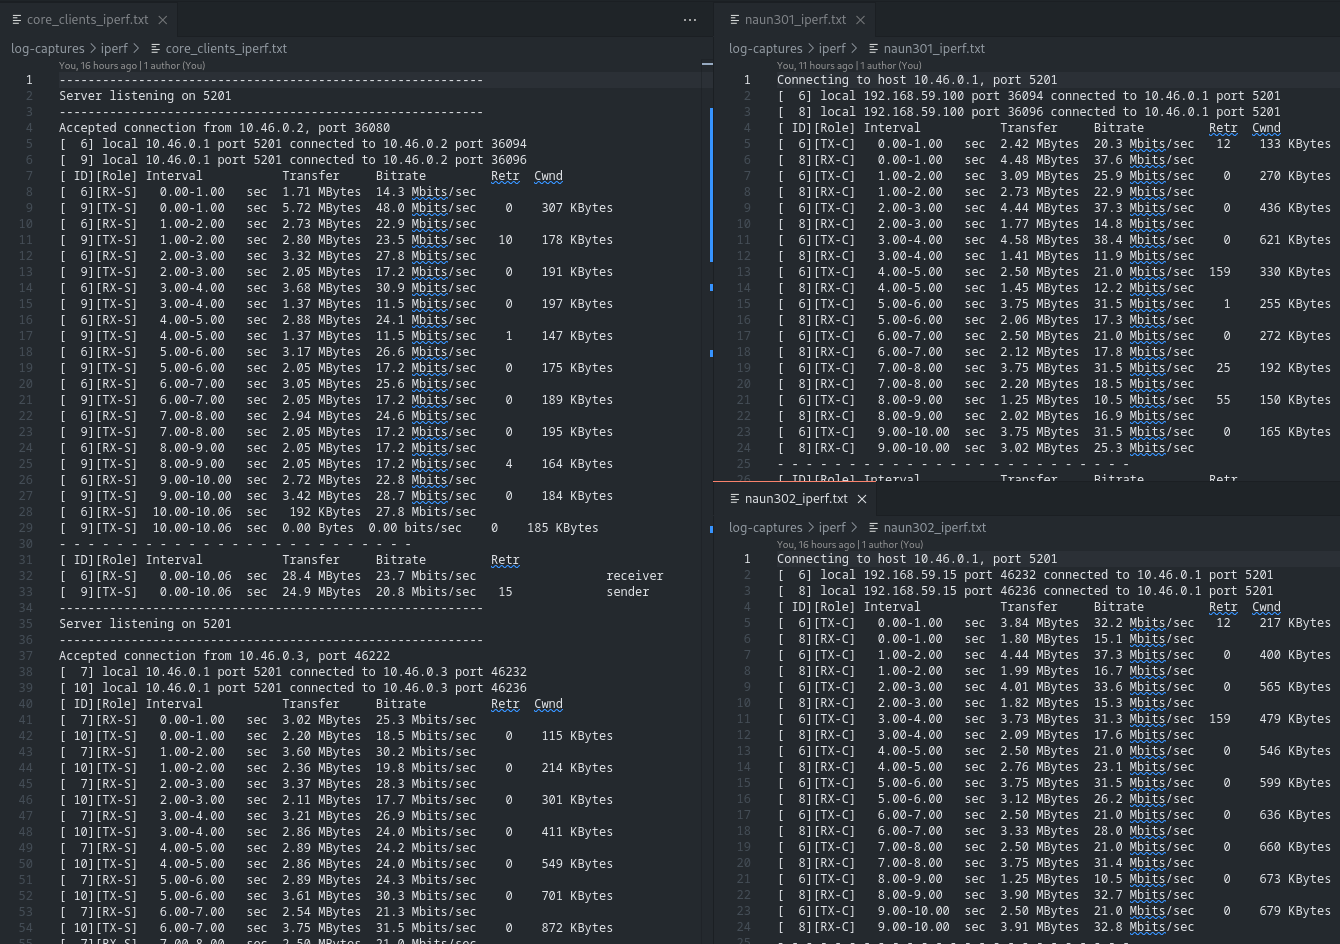
\includegraphics[width=1\linewidth]{figs/iperf_naun3_to_core.png}
    \caption{\texttt{iperf3} session between \acp{NAUN3} and \ac{5GC}}
    \label{fig:iperf_naun3_to_core}
\end{figure}

The \texttt{iperf3} tests further validated traffic isolation and mapping. As seen in the Figure \ref{fig:iperf_naun3_to_core}, it shows the \texttt{iperf3} server on \texttt{10.46.0.1} (on the left) accepting connections from two different source \acp{IP}: \texttt{10.46.0.2} and \texttt{10.46.0.3}. These correspond to the unique \ac{PDU} session \acp{IP} assigned to \texttt{naun301} and \texttt{naun302} respectively. This confirms that traffic from each \ac{NAUN3} device is correctly mapped to its dedicated \ac{PDU} session and is identifiable by this unique \ac{PDU} session \ac{IP} at the N6 network.

\begin{figure}
    \centering
    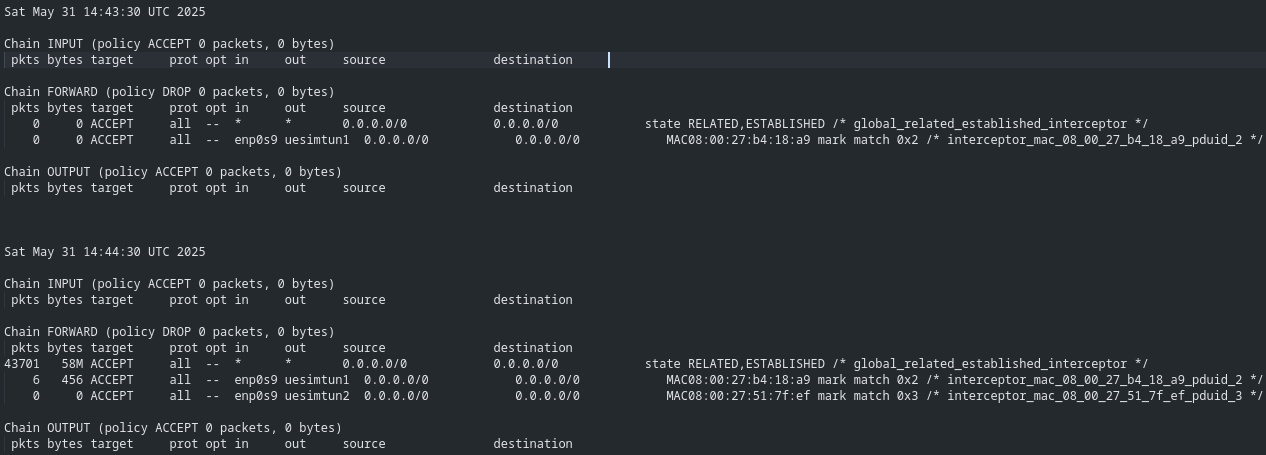
\includegraphics[width=1\linewidth]{figs/iptable_mapping_rules.png}
    \caption{\texttt{iptables} mapping rules and tables for segregating traffic}
    \label{fig:iptable_mapping_rules}
\end{figure}

Also, Figure \ref{fig:iptable_mapping_rules} shows the dynamic application of \texttt{iptables FORWARD} rules and \texttt{ip rule}/\texttt{ip route} entries. For instance, at 14:43:30 \ac{UTC} (after \texttt{naun301} connects), rules are present for \ac{MAC} \texttt{08:00:27:b4:18:a9} (\ac{naun301}) to use \ac{PDU} ID 2 (interface \texttt{uesimtun1}). By 14:44:30 \ac{UTC} (after \texttt{naun302} connects), additional rules appear for \ac{MAC} \texttt{08:00:27:51:7f:ef} (\texttt{naun302}) to use \ac{PDU} ID 3 (interface \texttt{uesimtun2}), while rules for \ac{PDU} ID 2 remain. This demonstrates the per-device rule application.

\begin{figure}
    \centering
    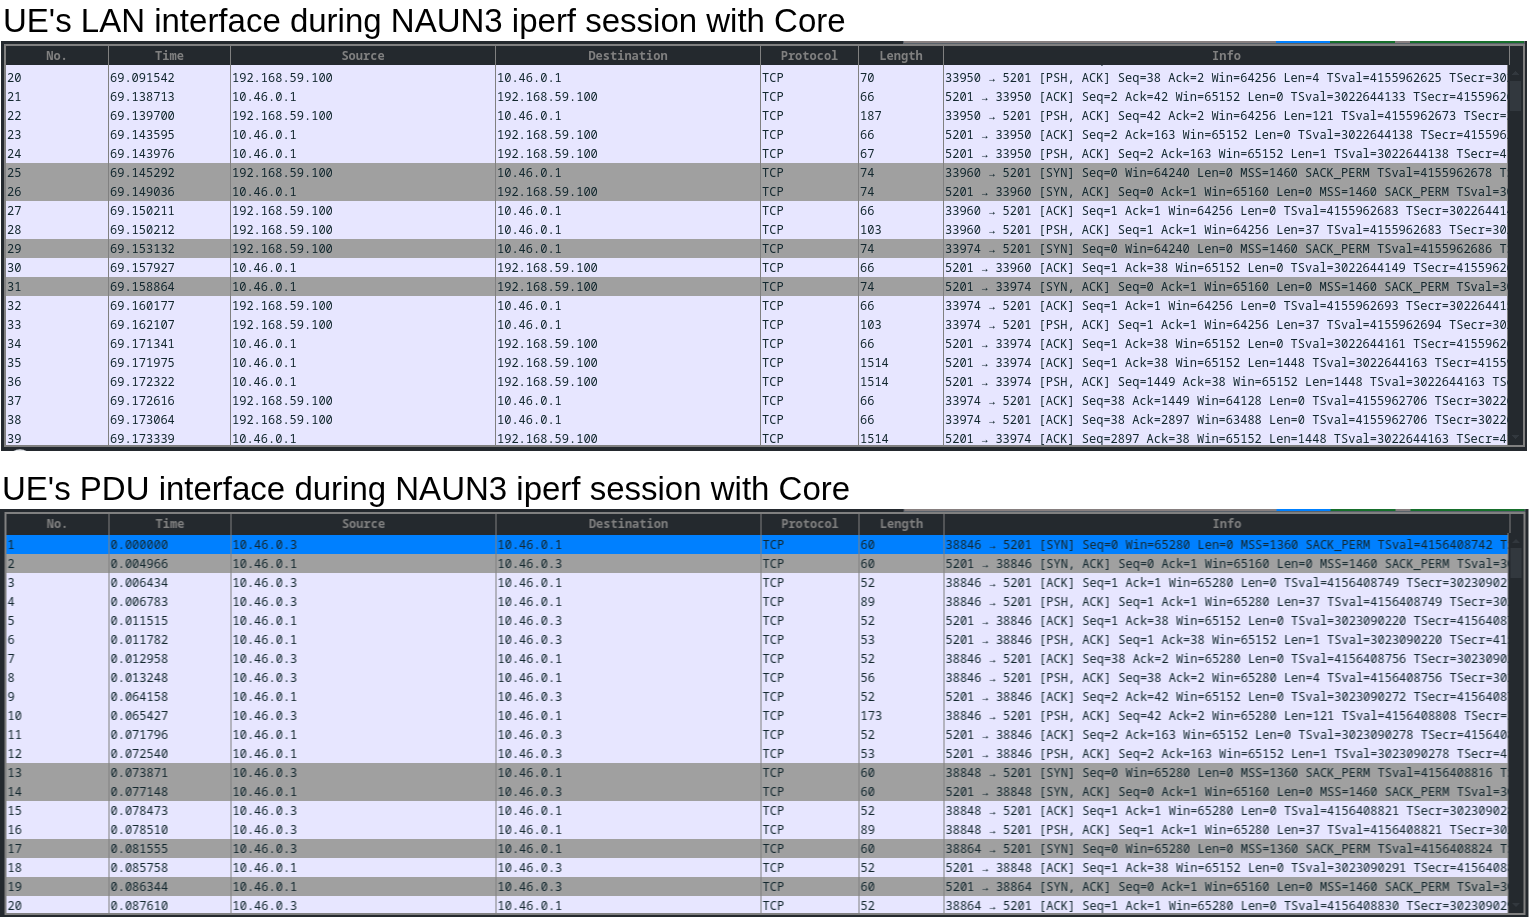
\includegraphics[width=1\linewidth]{figs/naun3_to_core_ue_view.png}
    \caption{\ac{NAUN3} to \ac{5GC} \texttt{iperf3} session, captured at the \ac{5G-RG} showing the mapping between the local address and \ac{PDU} session address}
    \label{fig:naun3_to_core_ue_view}
\end{figure}

The Wireshark capture in Figure \ref{fig:naun3_to_core_ue_view} visually confirms this: traffic on the \ac{5G-RG}'s \ac{LAN} interface shows the \ac{NAUN3}'s local \ac{IP} (e.g., \texttt{192.168.59.100}), while on the corresponding \ac{PDU} session tunnel interface (\texttt{uesimtunX}), the source \ac{IP} is the \ac{PDU} session's \ac{5GC}-assigned \ac{IP} (e.g., \texttt{10.46.0.3})

\subsection{Lifecycle Management (Device Disconnection)}

The logs demonstrate correct resource cleanup when \texttt{naun301} (associated with \ac{PDU} Session2, \ac{IP} \texttt{10.46.0.2}, interface \texttt{uesimtun1}) disconnects:

\begin{figure}
    \centering
    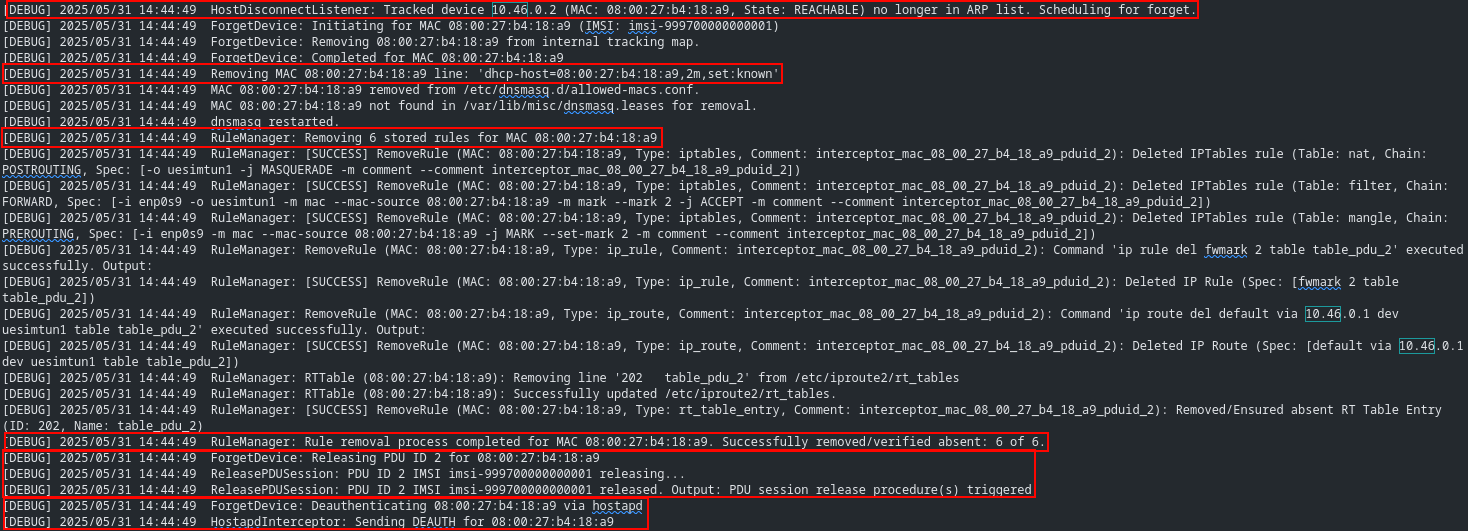
\includegraphics[width=1\linewidth]{figs/naun3_removed.png}
    \caption{\texttt{naun301} disconnected and \ac{5G-RG}'s \texttt{interceptor} proceeds to deauthenticating it, removing traffic mapping rules for it, and releasing it's dedicated \ac{PDU} session.}
    \label{fig:naun3_removed}
\end{figure}

\begin{itemize}
    \item \texttt{interceptor} (around 14:44:49 \ac{UTC}) logs, according to Figure \ref{fig:naun3_removed}: \textttt{"Tracked device 10.46.0.2 (MAC: 08:00:27:b4:18:a9, State: REACHABLE) no longer in ARP list. Scheduling for forget."} This is followed by logs indicating removal from \texttt{allowedDevices}, deauthentication via \texttt{hostapd}, removal of \texttt{iptables} rules, and \ac{PDU} session release for \ac{PDU} ID 2.

    \begin{figure}
        \centering
        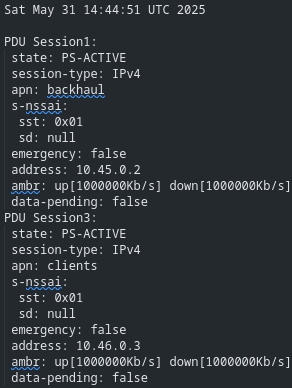
\includegraphics[width=0.20\linewidth]{figs/nr-cli_ps-list.png}
        \caption{\ac{PDU} session listing from UERANSIM}
        \label{fig:nr-cli_ps-list}
    \end{figure}

    \item According to Figure \ref{fig:nr-cli_ps-list}, at 14:44:51 \ac{UTC}, \ac{PDU} Session2 (\ac{IP} \texttt{10.46.0.2}) is no longer listed, while \ac{PDU} Session1 (\texttt{backhaul}) and \ac{PDU} Session3 (for \texttt{naun302}, \ac{IP} \texttt{10.46.0.3}) remain active.

    \begin{figure}
        \centering
        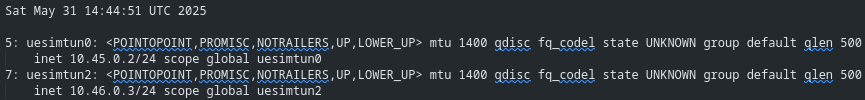
\includegraphics[width=1\linewidth]{figs/ue_pdu_sessions_nics_release.png}
        \caption{\ac{PDU} binded network interfaces after \texttt{uesimtun1} removal}
        \label{fig:ue_pdu_sessions_nics_release}
    \end{figure}
    
    \item Figure \ref{figs:ue_pdu_sessions_nics_release} also confirms that by 14:44:51 \ac{UTC}, the \texttt{uesimtun1} interface (associated with \texttt{10.46.0.2}) is gone, while \texttt{uesimtun0} and \texttt{uesimtun2} persist.

    \begin{figure}
        \centering
        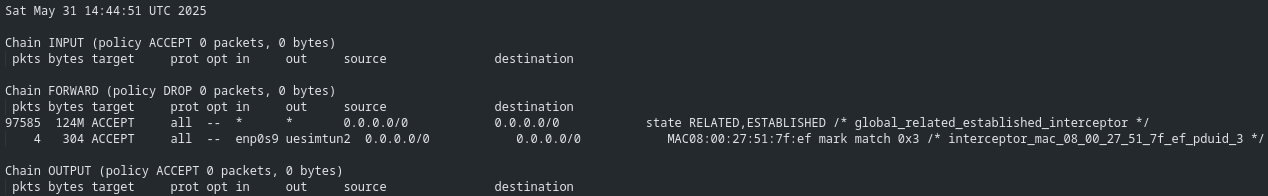
\includegraphics[width=1\linewidth]{figs/ue_naun3_to_pdu_mapping_rules.png}
        \caption{Mapping rules after \texttt{naun301} disconnect and \ac{PDU} Session2 release}
        \label{fig:ue_naun3_to_pdu_mapping_rules}
    \end{figure}

    \item Lastly, Figure \ref{figs:ue_naun3_to_pdu_mapping_rules} also hows that at 14:44:51 \ac{UTC}, the \texttt{iptables} \texttt{FORWARD} rule for \ac{MAC} \texttt{08:00:27:b4:18:a9} (\ac{PDU} ID 2) has been removed, while the rule for \ac{MAC} \texttt{08:00:27:51:7f:ef} (\ac{PDU} ID 3) remains.
\end{itemize}

These results collectively demonstrate that the proposed mechanisms for \ac{NAUN3} device authentication, proxy identity creation via dedicated \ac{PDU} sessions, per-device traffic mapping and \ac{NAT}, and lifecycle management function correctly within the simulated environment.

\section{Security Evaluation}

The security aspects of the solution were evaluated qualitatively based on the implemented mechanisms and observations from the test scenarios.

\begin{itemize}
    \item \textbf{\ac{EAP-TLS} Authentication Integrity:} The logs from \texttt{wpa\_supplicant} in the \acs{NAUN3}, \texttt{hostapd}, and FreeRADIUS consistently show the successful completion of the \ac{EAP-TLS} handshake. This includes the exchange of certificates and the mutual verification steps inherent to the protocol. For instance, FreeRADIUS logs details like \texttt{"eap\_tls: (TLS) Connection Established"} and \texttt{"eap: Sending EAP Success"}. This provides confidence that the local authentication of \ac{NAUN3} devices is cryptographically secured as per \ac{EAP-TLS} standards.

    \item{
        \textbf{Traffic Segregation (Control vs. User Plane):}
        \begin{itemize}
            \item In Figure \ref{fig:RADIUS_traffic_via_backhaul} a Wireshark capture clearly shows \ac{RADIUS} packets (\ac{UDP} port 1812), which carry the \ac{EAP} authentication messages, being exchanged between the \ac{5G-RG}'s \texttt{backhaul} \ac{PDU} session \ac{IP} (\texttt{10.45.0.2}) and the FreeRADIUS server's \ac{IP} (\texttt{10.45.0.1}). This confirms that sensitive authentication control plane traffic is isolated to the dedicated \texttt{backhaul} \ac{DNN}.

            \begin{figure}
                \centering
                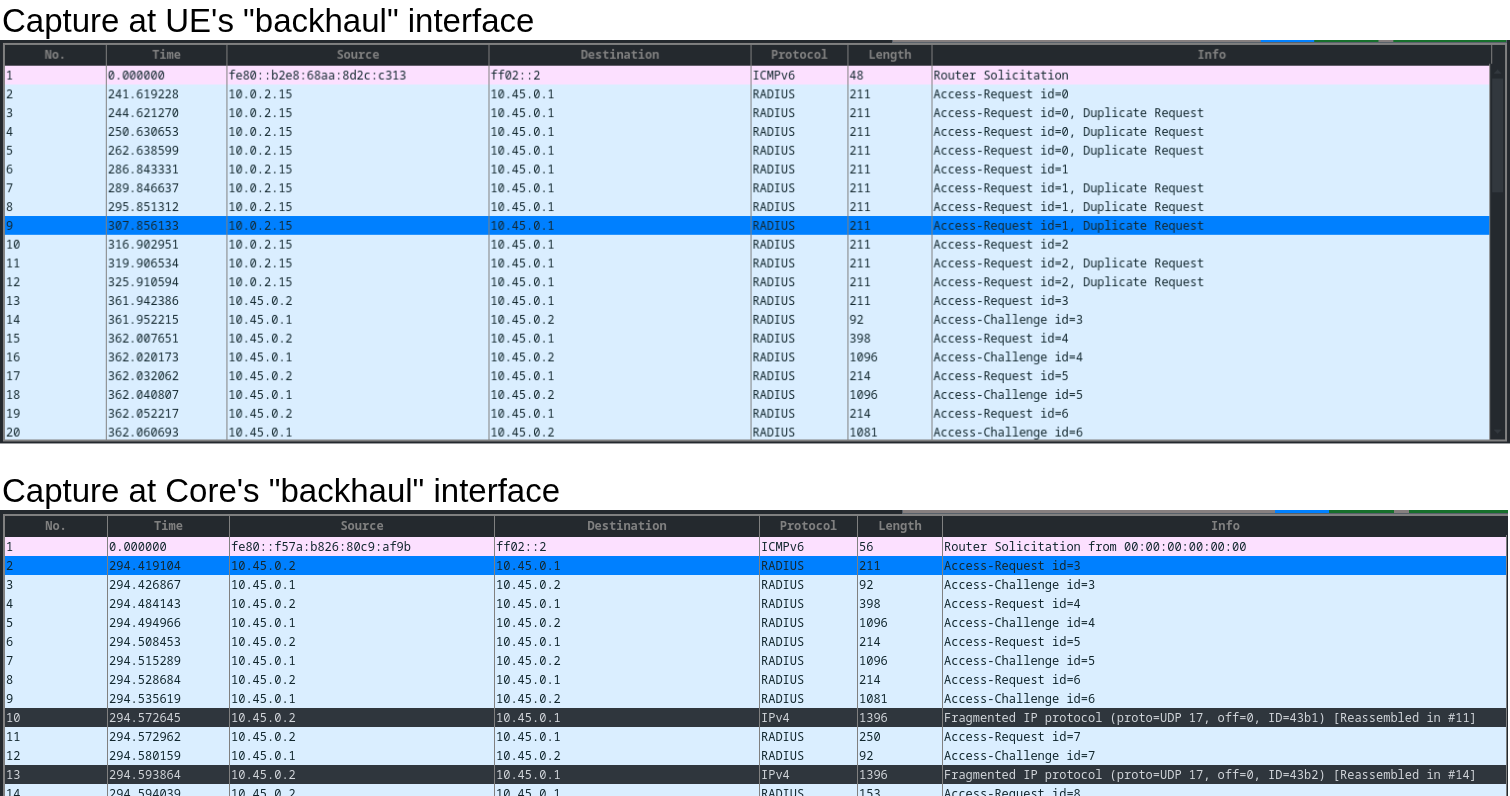
\includegraphics[width=0.75\linewidth]{figs/RADIUS_traffic_via_backhaul.png}
                \caption{\ac{RADIUS} traffic captured at \texttt{backhaul} channel via Wireshark}
                \label{fig:RADIUS_traffic_via_backhaul}
            \end{figure}

            \item The \texttt{hostapd} log (see Listing \ref{lst:hostapd_fail} ) further details the \ac{RADIUS} exchange, initially attempting to send from a default system \ac{IP} (e.g., \texttt{10.0.2.15}) and failing (evident by retransmissions), then succeeding once the \texttt{own\_ip\_addr} (\texttt{10.45.0.2} - the \texttt{backhaul} \ac{PDU} session \ac{IP}) is correctly used. This highlights the correct binding and use of the \texttt{backhaul} \ac{PDU} for \ac{RADIUS}.

\begin{lstlisting}[caption=hostapd failing due to wrong local address,label={lst:hostapd_fail}]
(...)
25 | 1748702388.755637: RADIUS local address: 10.0.2.15:42579
(...)
216| 1748702566.372520: RADIUS local address: 10.45.0.2:50371
(...)
\end{lstlisting}

            \item Conversely, user plane traffic from \ac{NAUN3} devices (e.g., \texttt{iperf3} data in Figure \ref{fig:iperf_naun3_to_core} and ping traffic in Figure \ref{fig:ping_gw}) is shown to originate from the \texttt{clients} \ac{DNN} \ac{IP} addresses (e.g., \texttt{10.46.0.2}, \texttt{10.46.0.3}) assigned to their respective \ac{PDU} sessions. This demonstrates effective segregation between the authentication control plane and the user data plane.
        \end{itemize}
    }
\end{itemize}

While these observations do not constitute a formal penetration test or vulnerability assessment, they confirm that the fundamental security design principles, strong local authentication via \ac{EAP-TLS}, segregation of control and user plane traffic via distinct \acp{DNN}, and abstraction of local \ac{NAUN3} device identities from the \ac{5GC}, are correctly implemented and operational within the test environment. The envisioned enhancement suggests a pathway to more integrated policy control if desired in future iterations.

\section{Performance Evaluation}

% Present the results related to the performance metrics defined earlier (e.g., authentication delay, computational overhead on involved network functions).

% Compare these results against baseline scenarios or standard procedures if possible.

\section{Discussion and Analysis}

The validation results presented in the preceding sections provide substantial evidence for the functional viability and integrity of the proposed framework for integrating Wi-Fi-only/\ac{NAUN3} devices into a \ac{5G} network. This discussion will interpret these findings in the context of the initial research objectives and requirements, compare the solution with standard \ac{3GPP} approaches, and acknowledge observed limitations.

\subsection{Interpretation of Results and Effectiveness in Meeting Requirements}

The primary goal was to devise a solution that allows \ac{NAUN3} devices, which lack \ac{5G} credentials, to securely access \ac{5G} network services with minimal impact on the devices themselves and the standard \ac{5GC}.

\begin{itemize}
    \item \textbf{Local Authentication (Requirement Met):} The successful \ac{EAP-TLS} authentication demonstrates that \ac{NAUN3} devices can be securely authenticated at the edge by the \ac{5G-RG} before any \ac{5G} resources are committed. This meets the requirement for a robust local authentication mechanism.

    \item \textbf{Individual Device Handling and Proxy Identity (Requirement Met):} The core concept of using a dedicated \ac{PDU} session as a proxy identity for each \ac{NAUN3} device was successfully implemented and validated. The \ac{UE} logs and Figures \ref{fig:ue_pdu_sessions_nics} and \ref{fig:iptable_mapping_rules} clearly show the dynamic creation of distinct \ac{PDU} sessions on the \texttt{clients} \ac{DNN}, each with a unique \ac{5GC}-assigned \ac{IP} address, corresponding to each authenticated \ac{NAUN3} device. The \texttt{interceptor} logs (see Figure \ref{fig:interceptor_eap_success}) further detail the interceptor application's role in orchestrating these \ac{PDU} session establishments via \texttt{nr-cli} upon \ac{EAP} success.

    \item \textbf{Traffic Mapping and Isolation (Requirement Met):} The \texttt{ping -R} tests (Figure \ref{fig:ping_gw}) and \texttt{iperf3} results (Figure \ref{fig:iperf_naun3_to_core} showing distinct source \acp{IP} \texttt{10.46.0.2} and \texttt{10.46.0.3}) confirm that traffic from each \ac{NAUN3} device is correctly \textit{NATted} and routed through its unique \ac{PDU} session. The Wireshark capture in Figure \ref{fig:naun3_to_core_ue_view} and the dynamic \texttt{iptables} rules in Figure \ref{fig:iptable_mapping_rules} further substantiate that the \ac{5G-RG} effectively maps local device traffic to its designated \ac{5G} \ac{PDU} session, ensuring traffic isolation.

    \item \textbf{Minimal Core Network and Device Impact (Requirement Met):} The solution operates without requiring any modifications to the \ac{NAUN3} devices beyond standard \ac{EAP-TLS} supplicant capabilities. The \ac{5GC} (Open5GS) interacts with the \ac{5G-RG} as a standard \ac{UE} requesting \ac{PDU} sessions; no changes to core \acp{NF} were needed beyond configuration (\acp{DNN}, subscriber data for the \ac{5G-RG}). This fulfills the critical requirement of minimal disruption.

    \item \textbf{Gateway-Centric Logic (Requirement Met):} All the specialized logic for \ac{NAUN3} authentication relay, \ac{PDU} session orchestration, and traffic mapping is concentrated within the \ac{5G-RG} (\texttt{ue} \ac{VM}), primarily within the custom \texttt{interceptor} application and configurations of \textt{hostapd} and \texttt{dnsmasq}.

    \item \textbf{Lifecycle Management (Requirement Met):} The logs in Figures \ref{fig:naun3_removed}, \ref{fig:ue_pdu_sessions_nics_release} and \ref{fig:ue_naun3_to_pdu_mapping_rules} demonstrate that upon simulated \ac{NAUN3} device disconnection, the \texttt{interceptor} correctly triggers local deauthentication, \ac{PDU} session termination, and cleanup of associated routing rules and \ac{DHCP} permissions.

    \item \textbf{Traffic Segregation (Requirement Met):} The capture seen in Figure \ref{fig:RADIUS_traffic_via_backhaul} confirm that authentication control plane traffic (\ac{RADIUS}/\ac{EAP}) is successfully segregated onto the \texttt{backhaul} \ac{DNN}, using the \ac{5G-RG}'s \ac{PDU} session \ac{IP} designated for this purpose, while \ac{NAUN3} user plane traffic utilizes the separate \texttt{clients} \ac{DNN} \ac{PDU} sessions.
\end{itemize}
%\chapter{Conclusion}%
\label{chapter:conclusion}

\begin{introduction}
Concluding the thesis, this chapter synthesizes the research conducted, summarizing the key findings and contributions toward integrating Wi-Fi-only devices in 5G environments. Re-visits the problem statement and research objectives, discusses the implications of the results, acknowledges the limitations encountered during the study, and proposes potential avenues for future research and development in this domain.
\end{introduction}

%%%%%%%%%%%%%%%%%%%%%%%%%%%%%%%%%%%%%%%%%%%%%%%%%%%%%%%
% End of Thesis text 
%%%%%%%%%%%%%%%%%%%%%%%%%%%%%%%%%%%%%%%%%%%%%%%%%%%%%%%

\backmatter

%%%%%%%%%%%%%%%%%%%%%%%%%%%%%%%%%%%%%%%%%%%%%%%%%%%%%%%
% Print all used references
%%%%%%%%%%%%%%%%%%%%%%%%%%%%%%%%%%%%%%%%%%%%%%%%%%%%%%%

\begingroup
\renewcommand{\bibfont}{\footnotesize}
% Redefine References name to Portuguese
% Change if you are using english
\defbibheading{bibliography}[References]{
	\chapter{#1}
}
\SingleSpacing
\setlength\bibitemsep{8pt}
\printbibliography[heading=bibliography]
\endgroup


%%%%%%%%%%%%%%%%%%%%%%%%%%%%%%%%%%%%%%%%%%%%%%%%%%%%%%%
% Load appendix
%%%%%%%%%%%%%%%%%%%%%%%%%%%%%%%%%%%%%%%%%%%%%%%%%%%%%%%

\mainmatterWithoutReset
\appendix

\chapter{Additional content}


\end{document}
